\documentclass[twoside]{book}

% Packages required by doxygen
\usepackage{fixltx2e}
\usepackage{calc}
\usepackage{doxygen}
\usepackage[export]{adjustbox} % also loads graphicx
\usepackage{graphicx}
\usepackage[utf8]{inputenc}
\usepackage{makeidx}
\usepackage{multicol}
\usepackage{multirow}
\PassOptionsToPackage{warn}{textcomp}
\usepackage{textcomp}
\usepackage[nointegrals]{wasysym}
\usepackage[table]{xcolor}

% Font selection
\usepackage[T1]{fontenc}
\usepackage[scaled=.90]{helvet}
\usepackage{courier}
\usepackage{amssymb}
\usepackage{sectsty}
\renewcommand{\familydefault}{\sfdefault}
\allsectionsfont{%
  \fontseries{bc}\selectfont%
  \color{darkgray}%
}
\renewcommand{\DoxyLabelFont}{%
  \fontseries{bc}\selectfont%
  \color{darkgray}%
}
\newcommand{\+}{\discretionary{\mbox{\scriptsize$\hookleftarrow$}}{}{}}

% Page & text layout
\usepackage{geometry}
\geometry{%
  a4paper,%
  top=2.5cm,%
  bottom=2.5cm,%
  left=2.5cm,%
  right=2.5cm%
}
\tolerance=750
\hfuzz=15pt
\hbadness=750
\setlength{\emergencystretch}{15pt}
\setlength{\parindent}{0cm}
\setlength{\parskip}{3ex plus 2ex minus 2ex}
\makeatletter
\renewcommand{\paragraph}{%
  \@startsection{paragraph}{4}{0ex}{-1.0ex}{1.0ex}{%
    \normalfont\normalsize\bfseries\SS@parafont%
  }%
}
\renewcommand{\subparagraph}{%
  \@startsection{subparagraph}{5}{0ex}{-1.0ex}{1.0ex}{%
    \normalfont\normalsize\bfseries\SS@subparafont%
  }%
}
\makeatother

% Headers & footers
\usepackage{fancyhdr}
\pagestyle{fancyplain}
\fancyhead[LE]{\fancyplain{}{\bfseries\thepage}}
\fancyhead[CE]{\fancyplain{}{}}
\fancyhead[RE]{\fancyplain{}{\bfseries\leftmark}}
\fancyhead[LO]{\fancyplain{}{\bfseries\rightmark}}
\fancyhead[CO]{\fancyplain{}{}}
\fancyhead[RO]{\fancyplain{}{\bfseries\thepage}}
\fancyfoot[LE]{\fancyplain{}{}}
\fancyfoot[CE]{\fancyplain{}{}}
\fancyfoot[RE]{\fancyplain{}{\bfseries\scriptsize Generated by Doxygen }}
\fancyfoot[LO]{\fancyplain{}{\bfseries\scriptsize Generated by Doxygen }}
\fancyfoot[CO]{\fancyplain{}{}}
\fancyfoot[RO]{\fancyplain{}{}}
\renewcommand{\footrulewidth}{0.4pt}
\renewcommand{\chaptermark}[1]{%
  \markboth{#1}{}%
}
\renewcommand{\sectionmark}[1]{%
  \markright{\thesection\ #1}%
}

% Indices & bibliography
\usepackage{natbib}
\usepackage[titles]{tocloft}
\setcounter{tocdepth}{3}
\setcounter{secnumdepth}{5}
\makeindex

% Packages requested by user
\usepackage{amsmath}
\usepackage{amssymb}
\usepackage{setspace}
\usepackage{esint}

% Hyperlinks (required, but should be loaded last)
\usepackage{ifpdf}
\ifpdf
  \usepackage[pdftex,pagebackref=true]{hyperref}
\else
  \usepackage[ps2pdf,pagebackref=true]{hyperref}
\fi
\hypersetup{%
  colorlinks=true,%
  linkcolor=blue,%
  citecolor=blue,%
  unicode%
}

% Custom commands
\newcommand{\clearemptydoublepage}{%
  \newpage{\pagestyle{empty}\cleardoublepage}%
}

\usepackage{caption}
\captionsetup{labelsep=space,justification=centering,font={bf},singlelinecheck=off,skip=4pt,position=top}

%===== C O N T E N T S =====

\begin{document}

% Titlepage & ToC
\hypersetup{pageanchor=false,
             bookmarksnumbered=true,
             pdfencoding=unicode
            }
\pagenumbering{roman}
\begin{titlepage}
\vspace*{7cm}
\begin{center}%
{\Large J\+A\+S\+PL \\[1ex]\large 0.\+2 }\\
\vspace*{1cm}
{\large Generated by Doxygen 1.8.11}\\
\end{center}
\end{titlepage}
\clearemptydoublepage
\tableofcontents
\clearemptydoublepage
\pagenumbering{arabic}
\hypersetup{pageanchor=true}

%--- Begin generated contents ---
\chapter{J\+A\+S\+PL ( Just another signal processing library )}
\label{md__home_bephillips2_Qt-Projects_JASPL_README}
\hypertarget{md__home_bephillips2_Qt-Projects_JASPL_README}{}
J\+A\+S\+PL is designed to perform one dimensional signal processing operations with an emphasis on G\+P\+G\+PU acceleration.

\section*{Dependencies}

\subsubsection*{Base}


\begin{DoxyItemize}
\item \href{http://www.boost.org/users/download/}{\tt Boost $>$= 1.\+62}
\item \href{http://www.fftw.org/download.html}{\tt fftw $>$= 3.\+3.\+5}
\item \href{https://github.com/dstahlke/gnuplot-iostream}{\tt gnuplot-\/iostream}
\end{DoxyItemize}

\subsubsection*{Compilier requirements}


\begin{DoxyItemize}
\item \mbox{[}Opem\+MP Support (e.\+g. G\+CC)\mbox{]}
\item \mbox{[}C++11 Compliant (e.\+g. G\+CC $>$= 4.\+8.\+2\mbox{]}
\end{DoxyItemize}

\subsubsection*{G\+PU Acceleration}

To use G\+PU accelerated functions you will need an Open\+CL implementation and cl\+F\+FT\+:


\begin{DoxyItemize}
\item \href{https://github.com/clMathLibraries/clFFT}{\tt cl\+F\+FT}
\end{DoxyItemize}

\subsection*{Authors}


\begin{DoxyItemize}
\item {\bfseries Benjamin J Phillips} -\/ {\itshape As part of the Axion Dark Matter Experiment ( A\+D\+MX )} 
\end{DoxyItemize}
\chapter{Hierarchical Index}
\section{Class Hierarchy}
This inheritance list is sorted roughly, but not completely, alphabetically\+:\begin{DoxyCompactList}
\item \contentsline{section}{gnuplotio\+:\+:Array\+Traits$<$ T, Enable $>$}{\pageref{classgnuplotio_1_1_array_traits}}{}
\item \contentsline{section}{gnuplotio\+:\+:Array\+Traits$<$ std\+:\+:pair$<$ T, U $>$ $>$}{\pageref{classgnuplotio_1_1_array_traits_3_01std_1_1pair_3_01_t_00_01_u_01_4_01_4}}{}
\item \contentsline{section}{gnuplotio\+:\+:Array\+Traits$<$ std\+:\+:pair$<$ T\+:\+:head\+\_\+type, T\+:\+:tail\+\_\+type $>$ $>$}{\pageref{classgnuplotio_1_1_array_traits}}{}
\begin{DoxyCompactList}
\item \contentsline{section}{gnuplotio\+:\+:Array\+Traits$<$ T, typename boost\+:\+:enable\+\_\+if$<$ boost\+:\+:mpl\+:\+:and\+\_\+$<$ is\+\_\+boost\+\_\+tuple$<$ T $>$, boost\+:\+:mpl\+:\+:not\+\_\+$<$ is\+\_\+boost\+\_\+tuple\+\_\+nulltype$<$ typename T\+:\+:tail\+\_\+type $>$ $>$ $>$ $>$\+:\+:type $>$}{\pageref{classgnuplotio_1_1_array_traits_3_01_t_00_01typename_01boost_1_1enable__if_3_01boost_1_1mpl_1_1a8de3a8fe198d85f7f5d28b9a2f5bf229}}{}
\end{DoxyCompactList}
\item \contentsline{section}{gnuplotio\+:\+:Array\+Traits$<$ T $>$}{\pageref{classgnuplotio_1_1_array_traits}}{}
\begin{DoxyCompactList}
\item \contentsline{section}{gnuplotio\+:\+:Array\+Traits$<$ T \& $>$}{\pageref{classgnuplotio_1_1_array_traits_3_01_t_01_6_01_4}}{}
\end{DoxyCompactList}
\item \contentsline{section}{gnuplotio\+:\+:Array\+Traits$<$ T\+:\+:head\+\_\+type $>$}{\pageref{classgnuplotio_1_1_array_traits}}{}
\begin{DoxyCompactList}
\item \contentsline{section}{gnuplotio\+:\+:Array\+Traits$<$ T, typename boost\+:\+:enable\+\_\+if$<$ boost\+:\+:mpl\+:\+:and\+\_\+$<$ is\+\_\+boost\+\_\+tuple$<$ T $>$, is\+\_\+boost\+\_\+tuple\+\_\+nulltype$<$ typename T\+:\+:tail\+\_\+type $>$ $>$ $>$\+:\+:type $>$}{\pageref{classgnuplotio_1_1_array_traits_3_01_t_00_01typename_01boost_1_1enable__if_3_01boost_1_1mpl_1_1ad3fa8e75dccbaae12a06d17831678a88}}{}
\end{DoxyCompactList}
\item \contentsline{section}{gnuplotio\+:\+:Array\+Traits\+Defaults$<$ V $>$}{\pageref{classgnuplotio_1_1_array_traits_defaults}}{}
\item \contentsline{section}{gnuplotio\+:\+:Array\+Traits\+Defaults$<$ T $>$}{\pageref{classgnuplotio_1_1_array_traits_defaults}}{}
\begin{DoxyCompactList}
\item \contentsline{section}{gnuplotio\+:\+:Array\+Traits$<$ T\mbox{[}N\mbox{]}$>$}{\pageref{classgnuplotio_1_1_array_traits_3_01_t[_n]_4}}{}
\end{DoxyCompactList}
\item \contentsline{section}{gnuplotio\+:\+:Array\+Traits\+Defaults$<$ T\+:\+:value\+\_\+type $>$}{\pageref{classgnuplotio_1_1_array_traits_defaults}}{}
\begin{DoxyCompactList}
\item \contentsline{section}{gnuplotio\+:\+:Array\+Traits$<$ T, typename boost\+:\+:enable\+\_\+if$<$ is\+\_\+like\+\_\+stl\+\_\+container$<$ T $>$ $>$\+:\+:type $>$}{\pageref{classgnuplotio_1_1_array_traits_3_01_t_00_01typename_01boost_1_1enable__if_3_01is__like__stl__co9e1736bbd08cd58c6993ab613a998887}}{}
\end{DoxyCompactList}
\item \contentsline{section}{gnuplotio\+:\+:Binary\+Sender$<$ T, Enable $>$}{\pageref{structgnuplotio_1_1_binary_sender}}{}
\item \contentsline{section}{gnuplotio\+:\+:Binary\+Sender$<$ std\+:\+:complex$<$ T $>$ $>$}{\pageref{structgnuplotio_1_1_binary_sender_3_01std_1_1complex_3_01_t_01_4_01_4}}{}
\item \contentsline{section}{gnuplotio\+:\+:Binary\+Sender$<$ std\+:\+:pair$<$ T, U $>$ $>$}{\pageref{structgnuplotio_1_1_binary_sender_3_01std_1_1pair_3_01_t_00_01_u_01_4_01_4}}{}
\item \contentsline{section}{gnuplotio\+:\+:Binary\+Sender$<$ T, typename boost\+:\+:enable\+\_\+if$<$ boost\+:\+:mpl\+:\+:and\+\_\+$<$ is\+\_\+boost\+\_\+tuple$<$ T $>$, boost\+:\+:mpl\+:\+:not\+\_\+$<$ is\+\_\+boost\+\_\+tuple\+\_\+nulltype$<$ typename T\+:\+:tail\+\_\+type $>$ $>$ $>$ $>$\+:\+:type $>$}{\pageref{structgnuplotio_1_1_binary_sender_3_01_t_00_01typename_01boost_1_1enable__if_3_01boost_1_1mpl_1_916ff7a758aa0b8917fd3b30ff275f06}}{}
\item \contentsline{section}{gnuplotio\+:\+:Binary\+Sender$<$ T, typename boost\+:\+:enable\+\_\+if$<$ boost\+:\+:mpl\+:\+:and\+\_\+$<$ is\+\_\+boost\+\_\+tuple$<$ T $>$, is\+\_\+boost\+\_\+tuple\+\_\+nulltype$<$ typename T\+:\+:tail\+\_\+type $>$ $>$ $>$\+:\+:type $>$}{\pageref{structgnuplotio_1_1_binary_sender_3_01_t_00_01typename_01boost_1_1enable__if_3_01boost_1_1mpl_1_29e1098ca8b7afc20f2ca0bc2e79506a}}{}
\item \contentsline{section}{gnuplotio\+:\+:Binfmt\+Sender$<$ T, Enable $>$}{\pageref{structgnuplotio_1_1_binfmt_sender}}{}
\item \contentsline{section}{gnuplotio\+:\+:Binfmt\+Sender$<$ boost\+:\+:int16\+\_\+t $>$}{\pageref{structgnuplotio_1_1_binfmt_sender_3_01boost_1_1int16__t_01_4}}{}
\item \contentsline{section}{gnuplotio\+:\+:Binfmt\+Sender$<$ boost\+:\+:int32\+\_\+t $>$}{\pageref{structgnuplotio_1_1_binfmt_sender_3_01boost_1_1int32__t_01_4}}{}
\item \contentsline{section}{gnuplotio\+:\+:Binfmt\+Sender$<$ boost\+:\+:int64\+\_\+t $>$}{\pageref{structgnuplotio_1_1_binfmt_sender_3_01boost_1_1int64__t_01_4}}{}
\item \contentsline{section}{gnuplotio\+:\+:Binfmt\+Sender$<$ boost\+:\+:int8\+\_\+t $>$}{\pageref{structgnuplotio_1_1_binfmt_sender_3_01boost_1_1int8__t_01_4}}{}
\item \contentsline{section}{gnuplotio\+:\+:Binfmt\+Sender$<$ boost\+:\+:uint16\+\_\+t $>$}{\pageref{structgnuplotio_1_1_binfmt_sender_3_01boost_1_1uint16__t_01_4}}{}
\item \contentsline{section}{gnuplotio\+:\+:Binfmt\+Sender$<$ boost\+:\+:uint32\+\_\+t $>$}{\pageref{structgnuplotio_1_1_binfmt_sender_3_01boost_1_1uint32__t_01_4}}{}
\item \contentsline{section}{gnuplotio\+:\+:Binfmt\+Sender$<$ boost\+:\+:uint64\+\_\+t $>$}{\pageref{structgnuplotio_1_1_binfmt_sender_3_01boost_1_1uint64__t_01_4}}{}
\item \contentsline{section}{gnuplotio\+:\+:Binfmt\+Sender$<$ boost\+:\+:uint8\+\_\+t $>$}{\pageref{structgnuplotio_1_1_binfmt_sender_3_01boost_1_1uint8__t_01_4}}{}
\item \contentsline{section}{gnuplotio\+:\+:Binfmt\+Sender$<$ double $>$}{\pageref{structgnuplotio_1_1_binfmt_sender_3_01double_01_4}}{}
\item \contentsline{section}{gnuplotio\+:\+:Binfmt\+Sender$<$ float $>$}{\pageref{structgnuplotio_1_1_binfmt_sender_3_01float_01_4}}{}
\item \contentsline{section}{gnuplotio\+:\+:Binfmt\+Sender$<$ std\+:\+:complex$<$ T $>$ $>$}{\pageref{structgnuplotio_1_1_binfmt_sender_3_01std_1_1complex_3_01_t_01_4_01_4}}{}
\item \contentsline{section}{gnuplotio\+:\+:Binfmt\+Sender$<$ std\+:\+:pair$<$ T, U $>$ $>$}{\pageref{structgnuplotio_1_1_binfmt_sender_3_01std_1_1pair_3_01_t_00_01_u_01_4_01_4}}{}
\item \contentsline{section}{gnuplotio\+:\+:Binfmt\+Sender$<$ T, typename boost\+:\+:enable\+\_\+if$<$ boost\+:\+:mpl\+:\+:and\+\_\+$<$ is\+\_\+boost\+\_\+tuple$<$ T $>$, boost\+:\+:mpl\+:\+:not\+\_\+$<$ is\+\_\+boost\+\_\+tuple\+\_\+nulltype$<$ typename T\+:\+:tail\+\_\+type $>$ $>$ $>$ $>$\+:\+:type $>$}{\pageref{structgnuplotio_1_1_binfmt_sender_3_01_t_00_01typename_01boost_1_1enable__if_3_01boost_1_1mpl_1_e9270e5cb86823566a0af3940aa51061}}{}
\item \contentsline{section}{gnuplotio\+:\+:Binfmt\+Sender$<$ T, typename boost\+:\+:enable\+\_\+if$<$ boost\+:\+:mpl\+:\+:and\+\_\+$<$ is\+\_\+boost\+\_\+tuple$<$ T $>$, is\+\_\+boost\+\_\+tuple\+\_\+nulltype$<$ typename T\+:\+:tail\+\_\+type $>$ $>$ $>$\+:\+:type $>$}{\pageref{structgnuplotio_1_1_binfmt_sender_3_01_t_00_01typename_01boost_1_1enable__if_3_01boost_1_1mpl_1_8c86f170c2e2969f5519817e5c367132}}{}
\item \contentsline{section}{gnuplotio\+:\+:Cast\+Int\+Text\+Sender$<$ T $>$}{\pageref{structgnuplotio_1_1_cast_int_text_sender}}{}
\item \contentsline{section}{gnuplotio\+:\+:Cast\+Int\+Text\+Sender$<$ char $>$}{\pageref{structgnuplotio_1_1_cast_int_text_sender}}{}
\begin{DoxyCompactList}
\item \contentsline{section}{gnuplotio\+:\+:Text\+Sender$<$ char $>$}{\pageref{structgnuplotio_1_1_text_sender_3_01char_01_4}}{}
\end{DoxyCompactList}
\item \contentsline{section}{gnuplotio\+:\+:Cast\+Int\+Text\+Sender$<$ signed char $>$}{\pageref{structgnuplotio_1_1_cast_int_text_sender}}{}
\begin{DoxyCompactList}
\item \contentsline{section}{gnuplotio\+:\+:Text\+Sender$<$ signed char $>$}{\pageref{structgnuplotio_1_1_text_sender_3_01signed_01char_01_4}}{}
\end{DoxyCompactList}
\item \contentsline{section}{gnuplotio\+:\+:Cast\+Int\+Text\+Sender$<$ unsigned char $>$}{\pageref{structgnuplotio_1_1_cast_int_text_sender}}{}
\begin{DoxyCompactList}
\item \contentsline{section}{gnuplotio\+:\+:Text\+Sender$<$ unsigned char $>$}{\pageref{structgnuplotio_1_1_text_sender_3_01unsigned_01char_01_4}}{}
\end{DoxyCompactList}
\item \contentsline{section}{gnuplotio\+:\+:Col\+Unwrap\+No}{\pageref{structgnuplotio_1_1_col_unwrap_no}}{}
\item \contentsline{section}{gnuplotio\+:\+:Col\+Unwrap\+Yes}{\pageref{structgnuplotio_1_1_col_unwrap_yes}}{}
\item \contentsline{section}{gnuplotio\+:\+:dont\+\_\+treat\+\_\+as\+\_\+stl\+\_\+container$<$ T $>$}{\pageref{structgnuplotio_1_1dont__treat__as__stl__container}}{}
\item \contentsline{section}{gnuplotio\+:\+:Error\+\_\+\+Inappropriate\+Deref}{\pageref{structgnuplotio_1_1_error___inappropriate_deref}}{}
\item \contentsline{section}{gnuplotio\+:\+:Error\+\_\+\+Was\+Not\+Container}{\pageref{structgnuplotio_1_1_error___was_not_container}}{}
\item \contentsline{section}{gnuplotio\+:\+:File\+Handle\+Wrapper}{\pageref{structgnuplotio_1_1_file_handle_wrapper}}{}
\begin{DoxyCompactList}
\item \contentsline{section}{gnuplotio\+:\+:Gnuplot}{\pageref{classgnuplotio_1_1_gnuplot}}{}
\end{DoxyCompactList}
\item \contentsline{section}{gnuplotio\+:\+:Flat\+Binary\+Sender$<$ T $>$}{\pageref{structgnuplotio_1_1_flat_binary_sender}}{}
\item \contentsline{section}{gnuplotio\+:\+:Flat\+Binary\+Sender$<$ boost\+:\+:int16\+\_\+t $>$}{\pageref{structgnuplotio_1_1_flat_binary_sender}}{}
\begin{DoxyCompactList}
\item \contentsline{section}{gnuplotio\+:\+:Binary\+Sender$<$ boost\+:\+:int16\+\_\+t $>$}{\pageref{structgnuplotio_1_1_binary_sender_3_01boost_1_1int16__t_01_4}}{}
\end{DoxyCompactList}
\item \contentsline{section}{gnuplotio\+:\+:Flat\+Binary\+Sender$<$ boost\+:\+:int32\+\_\+t $>$}{\pageref{structgnuplotio_1_1_flat_binary_sender}}{}
\begin{DoxyCompactList}
\item \contentsline{section}{gnuplotio\+:\+:Binary\+Sender$<$ boost\+:\+:int32\+\_\+t $>$}{\pageref{structgnuplotio_1_1_binary_sender_3_01boost_1_1int32__t_01_4}}{}
\end{DoxyCompactList}
\item \contentsline{section}{gnuplotio\+:\+:Flat\+Binary\+Sender$<$ boost\+:\+:int64\+\_\+t $>$}{\pageref{structgnuplotio_1_1_flat_binary_sender}}{}
\begin{DoxyCompactList}
\item \contentsline{section}{gnuplotio\+:\+:Binary\+Sender$<$ boost\+:\+:int64\+\_\+t $>$}{\pageref{structgnuplotio_1_1_binary_sender_3_01boost_1_1int64__t_01_4}}{}
\end{DoxyCompactList}
\item \contentsline{section}{gnuplotio\+:\+:Flat\+Binary\+Sender$<$ boost\+:\+:int8\+\_\+t $>$}{\pageref{structgnuplotio_1_1_flat_binary_sender}}{}
\begin{DoxyCompactList}
\item \contentsline{section}{gnuplotio\+:\+:Binary\+Sender$<$ boost\+:\+:int8\+\_\+t $>$}{\pageref{structgnuplotio_1_1_binary_sender_3_01boost_1_1int8__t_01_4}}{}
\end{DoxyCompactList}
\item \contentsline{section}{gnuplotio\+:\+:Flat\+Binary\+Sender$<$ boost\+:\+:uint16\+\_\+t $>$}{\pageref{structgnuplotio_1_1_flat_binary_sender}}{}
\begin{DoxyCompactList}
\item \contentsline{section}{gnuplotio\+:\+:Binary\+Sender$<$ boost\+:\+:uint16\+\_\+t $>$}{\pageref{structgnuplotio_1_1_binary_sender_3_01boost_1_1uint16__t_01_4}}{}
\end{DoxyCompactList}
\item \contentsline{section}{gnuplotio\+:\+:Flat\+Binary\+Sender$<$ boost\+:\+:uint32\+\_\+t $>$}{\pageref{structgnuplotio_1_1_flat_binary_sender}}{}
\begin{DoxyCompactList}
\item \contentsline{section}{gnuplotio\+:\+:Binary\+Sender$<$ boost\+:\+:uint32\+\_\+t $>$}{\pageref{structgnuplotio_1_1_binary_sender_3_01boost_1_1uint32__t_01_4}}{}
\end{DoxyCompactList}
\item \contentsline{section}{gnuplotio\+:\+:Flat\+Binary\+Sender$<$ boost\+:\+:uint64\+\_\+t $>$}{\pageref{structgnuplotio_1_1_flat_binary_sender}}{}
\begin{DoxyCompactList}
\item \contentsline{section}{gnuplotio\+:\+:Binary\+Sender$<$ boost\+:\+:uint64\+\_\+t $>$}{\pageref{structgnuplotio_1_1_binary_sender_3_01boost_1_1uint64__t_01_4}}{}
\end{DoxyCompactList}
\item \contentsline{section}{gnuplotio\+:\+:Flat\+Binary\+Sender$<$ boost\+:\+:uint8\+\_\+t $>$}{\pageref{structgnuplotio_1_1_flat_binary_sender}}{}
\begin{DoxyCompactList}
\item \contentsline{section}{gnuplotio\+:\+:Binary\+Sender$<$ boost\+:\+:uint8\+\_\+t $>$}{\pageref{structgnuplotio_1_1_binary_sender_3_01boost_1_1uint8__t_01_4}}{}
\end{DoxyCompactList}
\item \contentsline{section}{gnuplotio\+:\+:Flat\+Binary\+Sender$<$ double $>$}{\pageref{structgnuplotio_1_1_flat_binary_sender}}{}
\begin{DoxyCompactList}
\item \contentsline{section}{gnuplotio\+:\+:Binary\+Sender$<$ double $>$}{\pageref{structgnuplotio_1_1_binary_sender_3_01double_01_4}}{}
\end{DoxyCompactList}
\item \contentsline{section}{gnuplotio\+:\+:Flat\+Binary\+Sender$<$ float $>$}{\pageref{structgnuplotio_1_1_flat_binary_sender}}{}
\begin{DoxyCompactList}
\item \contentsline{section}{gnuplotio\+:\+:Binary\+Sender$<$ float $>$}{\pageref{structgnuplotio_1_1_binary_sender_3_01float_01_4}}{}
\end{DoxyCompactList}
\item \contentsline{section}{gnuplotio\+:\+:Float\+Text\+Sender$<$ T $>$}{\pageref{structgnuplotio_1_1_float_text_sender}}{}
\item \contentsline{section}{gnuplotio\+:\+:Float\+Text\+Sender$<$ double $>$}{\pageref{structgnuplotio_1_1_float_text_sender}}{}
\begin{DoxyCompactList}
\item \contentsline{section}{gnuplotio\+:\+:Text\+Sender$<$ double $>$}{\pageref{structgnuplotio_1_1_text_sender_3_01double_01_4}}{}
\end{DoxyCompactList}
\item \contentsline{section}{gnuplotio\+:\+:Float\+Text\+Sender$<$ float $>$}{\pageref{structgnuplotio_1_1_float_text_sender}}{}
\begin{DoxyCompactList}
\item \contentsline{section}{gnuplotio\+:\+:Text\+Sender$<$ float $>$}{\pageref{structgnuplotio_1_1_text_sender_3_01float_01_4}}{}
\end{DoxyCompactList}
\item \contentsline{section}{gnuplotio\+:\+:Float\+Text\+Sender$<$ long double $>$}{\pageref{structgnuplotio_1_1_float_text_sender}}{}
\begin{DoxyCompactList}
\item \contentsline{section}{gnuplotio\+:\+:Text\+Sender$<$ long double $>$}{\pageref{structgnuplotio_1_1_text_sender_3_01long_01double_01_4}}{}
\end{DoxyCompactList}
\item \contentsline{section}{gnuplotio\+:\+:Gnuplot\+Feedback}{\pageref{classgnuplotio_1_1_gnuplot_feedback}}{}
\item \contentsline{section}{jaspl\+:\+:has\+\_\+accessor$<$ T $>$}{\pageref{classjaspl_1_1has__accessor}}{}
\item \contentsline{section}{jaspl\+:\+:has\+\_\+begin\+\_\+end$<$ T $>$}{\pageref{structjaspl_1_1has__begin__end}}{}
\item \contentsline{section}{jaspl\+:\+:has\+\_\+const\+\_\+iterator$<$ T $>$}{\pageref{structjaspl_1_1has__const__iterator}}{}
\item \contentsline{section}{jaspl\+:\+:has\+\_\+data$<$ T $>$}{\pageref{classjaspl_1_1has__data}}{}
\item \contentsline{section}{jaspl\+:\+:has\+\_\+data2$<$ T, Args $>$}{\pageref{classjaspl_1_1has__data2}}{}
\item \contentsline{section}{jaspl\+:\+:has\+\_\+size$<$ T $>$}{\pageref{classjaspl_1_1has__size}}{}
\item \contentsline{section}{gnuplotio\+:\+:is\+\_\+boost\+\_\+tuple$<$ T $>$}{\pageref{structgnuplotio_1_1is__boost__tuple}}{}
\item \contentsline{section}{gnuplotio\+:\+:is\+\_\+boost\+\_\+tuple\+\_\+nulltype$<$ T $>$}{\pageref{structgnuplotio_1_1is__boost__tuple__nulltype}}{}
\item \contentsline{section}{gnuplotio\+:\+:is\+\_\+boost\+\_\+tuple\+\_\+nulltype$<$ boost\+:\+:tuples\+:\+:null\+\_\+type $>$}{\pageref{structgnuplotio_1_1is__boost__tuple__nulltype_3_01boost_1_1tuples_1_1null__type_01_4}}{}
\item \contentsline{section}{gnuplotio\+:\+:is\+\_\+like\+\_\+stl\+\_\+container$<$ T $>$}{\pageref{structgnuplotio_1_1is__like__stl__container}}{}
\item \contentsline{section}{jaspl\+:\+:is\+\_\+stdlib\+\_\+container$<$ T $>$}{\pageref{structjaspl_1_1is__stdlib__container}}{}
\item \contentsline{section}{gnuplotio\+:\+:Iterator\+Range$<$ TI, TV $>$}{\pageref{classgnuplotio_1_1_iterator_range}}{}
\item \contentsline{section}{jaspl\+:\+:J\+F\+FT}{\pageref{classjaspl_1_1_j_f_f_t}}{}
\item \contentsline{section}{jaspl\+:\+:J\+F\+F\+T\+Unit\+Test$<$ T $>$}{\pageref{classjaspl_1_1_j_f_f_t_unit_test}}{}
\item \contentsline{section}{jaspl\+:\+:J\+Filter}{\pageref{classjaspl_1_1_j_filter}}{}
\item \contentsline{section}{jaspl\+:\+:j\+Filter\+Unit\+Test$<$ T $>$}{\pageref{classjaspl_1_1j_filter_unit_test}}{}
\item \contentsline{section}{J\+Non\+Linear\+Filter}{\pageref{class_j_non_linear_filter}}{}
\item \contentsline{section}{jaspl\+:\+:J\+Vector$<$ F $>$}{\pageref{classjaspl_1_1_j_vector}}{}
\item length\+\_\+error\begin{DoxyCompactList}
\item \contentsline{section}{gnuplotio\+:\+:plotting\+\_\+empty\+\_\+container}{\pageref{classgnuplotio_1_1plotting__empty__container}}{}
\end{DoxyCompactList}
\item \contentsline{section}{gnuplotio\+:\+:Mode1D}{\pageref{structgnuplotio_1_1_mode1_d}}{}
\item \contentsline{section}{gnuplotio\+:\+:Mode1\+D\+Unwrap}{\pageref{structgnuplotio_1_1_mode1_d_unwrap}}{}
\item \contentsline{section}{gnuplotio\+:\+:Mode2D}{\pageref{structgnuplotio_1_1_mode2_d}}{}
\item \contentsline{section}{gnuplotio\+:\+:Mode2\+D\+Unwrap}{\pageref{structgnuplotio_1_1_mode2_d_unwrap}}{}
\item \contentsline{section}{gnuplotio\+:\+:Mode\+Auto}{\pageref{structgnuplotio_1_1_mode_auto}}{}
\item \contentsline{section}{gnuplotio\+:\+:Mode\+Auto\+Decoder$<$ T, Enable $>$}{\pageref{structgnuplotio_1_1_mode_auto_decoder}}{}
\item \contentsline{section}{gnuplotio\+:\+:Mode\+Binary}{\pageref{structgnuplotio_1_1_mode_binary}}{}
\item \contentsline{section}{gnuplotio\+:\+:Mode\+Binfmt}{\pageref{structgnuplotio_1_1_mode_binfmt}}{}
\item \contentsline{section}{gnuplotio\+:\+:Mode\+Size}{\pageref{structgnuplotio_1_1_mode_size}}{}
\item \contentsline{section}{gnuplotio\+:\+:Mode\+Text}{\pageref{structgnuplotio_1_1_mode_text}}{}
\item \contentsline{section}{jaspl\+:\+:ocl\+:\+:Open\+C\+L\+Base}{\pageref{classjaspl_1_1ocl_1_1_open_c_l_base}}{}
\begin{DoxyCompactList}
\item \contentsline{section}{jaspl\+:\+:ocl\+:\+:Task\+Item}{\pageref{classjaspl_1_1ocl_1_1_task_item}}{}
\begin{DoxyCompactList}
\item \contentsline{section}{jaspl\+:\+:ocl\+:\+:F\+FT$<$ T $>$}{\pageref{classjaspl_1_1ocl_1_1_f_f_t}}{}
\begin{DoxyCompactList}
\item \contentsline{section}{jaspl\+:\+:ocl\+:\+:Power\+Spectrum$<$ T $>$}{\pageref{classjaspl_1_1ocl_1_1_power_spectrum}}{}
\end{DoxyCompactList}
\item \contentsline{section}{jaspl\+:\+:ocl\+:\+:Linear\+Convolution$<$ T $>$}{\pageref{classjaspl_1_1ocl_1_1_linear_convolution}}{}
\item \contentsline{section}{jaspl\+:\+:ocl\+:\+:Non\+Linear\+Convolution$<$ T $>$}{\pageref{classjaspl_1_1ocl_1_1_non_linear_convolution}}{}
\item \contentsline{section}{jaspl\+:\+:ocl\+:\+:Rebin}{\pageref{classjaspl_1_1ocl_1_1_rebin}}{}
\item \contentsline{section}{jaspl\+:\+:ocl\+:\+:Scalar\+Add$<$ T $>$}{\pageref{classjaspl_1_1ocl_1_1_scalar_add}}{}
\item \contentsline{section}{jaspl\+:\+:ocl\+:\+:Scalar\+Multiply$<$ T $>$}{\pageref{classjaspl_1_1ocl_1_1_scalar_multiply}}{}
\end{DoxyCompactList}
\item \contentsline{section}{jaspl\+:\+:ocl\+:\+:Task\+Queue\+Base}{\pageref{classjaspl_1_1ocl_1_1_task_queue_base}}{}
\begin{DoxyCompactList}
\item \contentsline{section}{jaspl\+:\+:ocl\+:\+:Task\+Queue$<$ T $>$}{\pageref{classjaspl_1_1ocl_1_1_task_queue}}{}
\item \contentsline{section}{jaspl\+:\+:ocl\+:\+:Task\+Queue$<$ T $\ast$ $>$}{\pageref{classjaspl_1_1ocl_1_1_task_queue_3_01_t_01_5_01_4}}{}
\end{DoxyCompactList}
\end{DoxyCompactList}
\item \contentsline{section}{gnuplotio\+:\+:Pair\+Of\+Range$<$ RT, RU $>$}{\pageref{classgnuplotio_1_1_pair_of_range}}{}
\item Q\+Main\+Window\begin{DoxyCompactList}
\item \contentsline{section}{J\+Chart}{\pageref{class_j_chart}}{}
\end{DoxyCompactList}
\item \contentsline{section}{jaspl\+:\+:Recurse\+Mean$<$ T $>$}{\pageref{classjaspl_1_1_recurse_mean}}{}
\item stream\begin{DoxyCompactList}
\item \contentsline{section}{gnuplotio\+:\+:Gnuplot}{\pageref{classgnuplotio_1_1_gnuplot}}{}
\end{DoxyCompactList}
\item \contentsline{section}{gnuplotio\+:\+:Text\+Sender$<$ T, Enable $>$}{\pageref{structgnuplotio_1_1_text_sender}}{}
\item \contentsline{section}{gnuplotio\+:\+:Text\+Sender$<$ std\+:\+:complex$<$ T $>$ $>$}{\pageref{structgnuplotio_1_1_text_sender_3_01std_1_1complex_3_01_t_01_4_01_4}}{}
\item \contentsline{section}{gnuplotio\+:\+:Text\+Sender$<$ std\+:\+:pair$<$ T, U $>$ $>$}{\pageref{structgnuplotio_1_1_text_sender_3_01std_1_1pair_3_01_t_00_01_u_01_4_01_4}}{}
\item \contentsline{section}{gnuplotio\+:\+:Text\+Sender$<$ T, typename boost\+:\+:enable\+\_\+if$<$ boost\+:\+:mpl\+:\+:and\+\_\+$<$ is\+\_\+boost\+\_\+tuple$<$ T $>$, boost\+:\+:mpl\+:\+:not\+\_\+$<$ is\+\_\+boost\+\_\+tuple\+\_\+nulltype$<$ typename T\+:\+:tail\+\_\+type $>$ $>$ $>$ $>$\+:\+:type $>$}{\pageref{structgnuplotio_1_1_text_sender_3_01_t_00_01typename_01boost_1_1enable__if_3_01boost_1_1mpl_1_1ad1ac3a3da167856c52be6ae54ba2c114}}{}
\item \contentsline{section}{gnuplotio\+:\+:Text\+Sender$<$ T, typename boost\+:\+:enable\+\_\+if$<$ boost\+:\+:mpl\+:\+:and\+\_\+$<$ is\+\_\+boost\+\_\+tuple$<$ T $>$, is\+\_\+boost\+\_\+tuple\+\_\+nulltype$<$ typename T\+:\+:tail\+\_\+type $>$ $>$ $>$\+:\+:type $>$}{\pageref{structgnuplotio_1_1_text_sender_3_01_t_00_01typename_01boost_1_1enable__if_3_01boost_1_1mpl_1_1ab6d6864cc1b3ed233c9f15134694f953}}{}
\item \contentsline{section}{gnuplotio\+:\+:type$<$ T $>$}{\pageref{structgnuplotio_1_1_mode_auto_decoder_3_01_t_00_01typename_01boost_1_1enable__if__c_3_01_07_arra33ab7f3325313485a7f29355d9a819fc}}{}
\item \contentsline{section}{gnuplotio\+:\+:type$<$ T $>$}{\pageref{structgnuplotio_1_1_mode_auto_decoder_3_01_t_00_01typename_01boost_1_1enable__if__c_3_01_07_arraea646779afc1e35efaeffcebe81e18a0}}{}
\item \contentsline{section}{gnuplotio\+:\+:type$<$ T $>$}{\pageref{structgnuplotio_1_1_mode_auto_decoder_3_01_t_00_01typename_01boost_1_1enable__if__c_3_01_07_arra8faa7fb46cef74a29a23f22c000e4a99}}{}
\item \contentsline{section}{gnuplotio\+:\+:Vec\+Of\+Range$<$ RT $>$}{\pageref{classgnuplotio_1_1_vec_of_range}}{}
\end{DoxyCompactList}

\chapter{Class Index}
\section{Class List}
Here are the classes, structs, unions and interfaces with brief descriptions\+:\begin{DoxyCompactList}
\item\contentsline{section}{\hyperlink{classjaspl_1_1ocl_1_1_f_f_t}{jaspl\+::ocl\+::\+F\+F\+T$<$ T $>$} }{\pageref{classjaspl_1_1ocl_1_1_f_f_t}}{}
\item\contentsline{section}{\hyperlink{classjaspl_1_1has__accessor}{jaspl\+::has\+\_\+accessor$<$ T $>$} }{\pageref{classjaspl_1_1has__accessor}}{}
\item\contentsline{section}{\hyperlink{structjaspl_1_1has__begin__end}{jaspl\+::has\+\_\+begin\+\_\+end$<$ T $>$} }{\pageref{structjaspl_1_1has__begin__end}}{}
\item\contentsline{section}{\hyperlink{structjaspl_1_1has__const__iterator}{jaspl\+::has\+\_\+const\+\_\+iterator$<$ T $>$} }{\pageref{structjaspl_1_1has__const__iterator}}{}
\item\contentsline{section}{\hyperlink{classjaspl_1_1has__data}{jaspl\+::has\+\_\+data$<$ T $>$} }{\pageref{classjaspl_1_1has__data}}{}
\item\contentsline{section}{\hyperlink{classjaspl_1_1has__data2}{jaspl\+::has\+\_\+data2$<$ T, Args $>$} }{\pageref{classjaspl_1_1has__data2}}{}
\item\contentsline{section}{\hyperlink{classjaspl_1_1has__size}{jaspl\+::has\+\_\+size$<$ T $>$} }{\pageref{classjaspl_1_1has__size}}{}
\item\contentsline{section}{\hyperlink{structjaspl_1_1is__stdlib__container}{jaspl\+::is\+\_\+stdlib\+\_\+container$<$ T $>$} }{\pageref{structjaspl_1_1is__stdlib__container}}{}
\item\contentsline{section}{\hyperlink{class_j_chart}{J\+Chart} }{\pageref{class_j_chart}}{}
\item\contentsline{section}{\hyperlink{classjaspl_1_1_j_f_f_t}{jaspl\+::\+J\+F\+F\+T$<$ T $>$} }{\pageref{classjaspl_1_1_j_f_f_t}}{}
\item\contentsline{section}{\hyperlink{classjaspl_1_1_j_filter}{jaspl\+::\+J\+Filter} }{\pageref{classjaspl_1_1_j_filter}}{}
\item\contentsline{section}{\hyperlink{classjaspl_1_1j_filter_unit_test}{jaspl\+::j\+Filter\+Unit\+Test$<$ T $>$} }{\pageref{classjaspl_1_1j_filter_unit_test}}{}
\item\contentsline{section}{\hyperlink{class_j_non_linear_filter}{J\+Non\+Linear\+Filter} }{\pageref{class_j_non_linear_filter}}{}
\item\contentsline{section}{\hyperlink{classjaspl_1_1_j_vector}{jaspl\+::\+J\+Vector$<$ F $>$} }{\pageref{classjaspl_1_1_j_vector}}{}
\item\contentsline{section}{\hyperlink{classjaspl_1_1ocl_1_1_linear_convolution}{jaspl\+::ocl\+::\+Linear\+Convolution$<$ T $>$} }{\pageref{classjaspl_1_1ocl_1_1_linear_convolution}}{}
\item\contentsline{section}{\hyperlink{classjaspl_1_1ocl_1_1_non_linear_convolution}{jaspl\+::ocl\+::\+Non\+Linear\+Convolution$<$ T $>$} }{\pageref{classjaspl_1_1ocl_1_1_non_linear_convolution}}{}
\item\contentsline{section}{\hyperlink{classjaspl_1_1ocl_1_1_open_c_l_base}{jaspl\+::ocl\+::\+Open\+C\+L\+Base} \\*Base class for every class that needs access to Open\+CL Platforms, Contexts or Devices }{\pageref{classjaspl_1_1ocl_1_1_open_c_l_base}}{}
\item\contentsline{section}{\hyperlink{classjaspl_1_1ouroborus}{jaspl\+::ouroborus$<$ T $>$} }{\pageref{classjaspl_1_1ouroborus}}{}
\item\contentsline{section}{\hyperlink{classjaspl_1_1_plotter}{jaspl\+::\+Plotter$<$ T $>$} }{\pageref{classjaspl_1_1_plotter}}{}
\item\contentsline{section}{\hyperlink{classjaspl_1_1ocl_1_1_power_spectrum}{jaspl\+::ocl\+::\+Power\+Spectrum$<$ T $>$} }{\pageref{classjaspl_1_1ocl_1_1_power_spectrum}}{}
\item\contentsline{section}{\hyperlink{classjaspl_1_1ocl_1_1_rebin}{jaspl\+::ocl\+::\+Rebin} }{\pageref{classjaspl_1_1ocl_1_1_rebin}}{}
\item\contentsline{section}{\hyperlink{classjaspl_1_1_recurse_mean}{jaspl\+::\+Recurse\+Mean$<$ T $>$} \\*Average together a (nearly) arbitrary number of container-\/like objects using the recursive definition of the expected value defined by\+: }{\pageref{classjaspl_1_1_recurse_mean}}{}
\item\contentsline{section}{\hyperlink{classjaspl_1_1ocl_1_1_scalar_add}{jaspl\+::ocl\+::\+Scalar\+Add$<$ T $>$} }{\pageref{classjaspl_1_1ocl_1_1_scalar_add}}{}
\item\contentsline{section}{\hyperlink{classjaspl_1_1ocl_1_1_scalar_multiply}{jaspl\+::ocl\+::\+Scalar\+Multiply$<$ T $>$} }{\pageref{classjaspl_1_1ocl_1_1_scalar_multiply}}{}
\item\contentsline{section}{\hyperlink{classjaspl_1_1ocl_1_1_task_item}{jaspl\+::ocl\+::\+Task\+Item} }{\pageref{classjaspl_1_1ocl_1_1_task_item}}{}
\item\contentsline{section}{\hyperlink{classjaspl_1_1ocl_1_1_task_queue}{jaspl\+::ocl\+::\+Task\+Queue$<$ T $>$} }{\pageref{classjaspl_1_1ocl_1_1_task_queue}}{}
\item\contentsline{section}{\hyperlink{classjaspl_1_1ocl_1_1_task_queue_3_01_t_01_5_01_4}{jaspl\+::ocl\+::\+Task\+Queue$<$ T $\ast$ $>$} }{\pageref{classjaspl_1_1ocl_1_1_task_queue_3_01_t_01_5_01_4}}{}
\item\contentsline{section}{\hyperlink{classjaspl_1_1ocl_1_1_task_queue_base}{jaspl\+::ocl\+::\+Task\+Queue\+Base} \\*The fundamental structure underlying all Open\+CL Functions }{\pageref{classjaspl_1_1ocl_1_1_task_queue_base}}{}
\end{DoxyCompactList}

\chapter{Class Documentation}
\hypertarget{classjaspl_1_1ocl_1_1_f_f_t}{}\section{jaspl\+:\+:ocl\+:\+:F\+FT$<$ T $>$ Class Template Reference}
\label{classjaspl_1_1ocl_1_1_f_f_t}\index{jaspl\+::ocl\+::\+F\+F\+T$<$ T $>$@{jaspl\+::ocl\+::\+F\+F\+T$<$ T $>$}}


Inheritance diagram for jaspl\+:\+:ocl\+:\+:F\+FT$<$ T $>$\+:\nopagebreak
\begin{figure}[H]
\begin{center}
\leavevmode
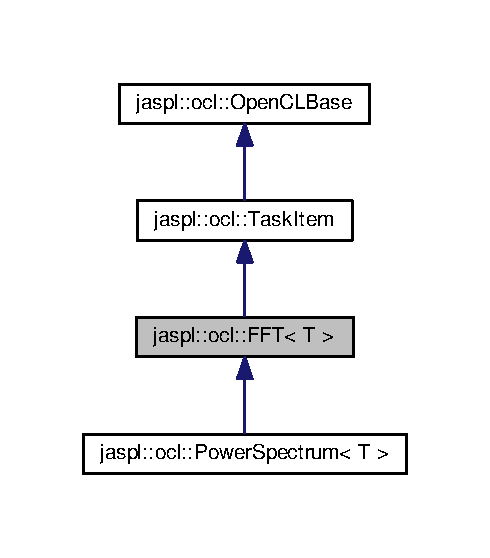
\includegraphics[width=235pt]{classjaspl_1_1ocl_1_1_f_f_t__inherit__graph}
\end{center}
\end{figure}


Collaboration diagram for jaspl\+:\+:ocl\+:\+:F\+FT$<$ T $>$\+:\nopagebreak
\begin{figure}[H]
\begin{center}
\leavevmode
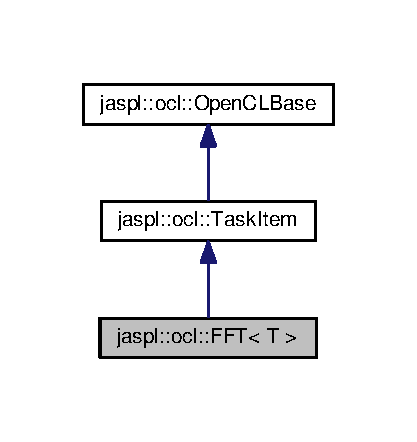
\includegraphics[width=200pt]{classjaspl_1_1ocl_1_1_f_f_t__coll__graph}
\end{center}
\end{figure}
\subsection*{Protected Member Functions}
\begin{DoxyCompactItemize}
\item 
void {\bfseries Trigger} ()\hypertarget{classjaspl_1_1ocl_1_1_f_f_t_a102a4328d7a30cc8ca8d08c907111fb2}{}\label{classjaspl_1_1ocl_1_1_f_f_t_a102a4328d7a30cc8ca8d08c907111fb2}

\item 
virtual void {\bfseries Set\+Signal} (cl\+::\+Buffer \&signal\+\_\+buff, uint sig\+\_\+size)\hypertarget{classjaspl_1_1ocl_1_1_f_f_t_ab38bdc5c38a82feaddb370f965295efd}{}\label{classjaspl_1_1ocl_1_1_f_f_t_ab38bdc5c38a82feaddb370f965295efd}

\item 
virtual cl\+::\+Buffer \& {\bfseries Processed\+Signal} ()\hypertarget{classjaspl_1_1ocl_1_1_f_f_t_aa03127efd639a389ec6869cc77fed978}{}\label{classjaspl_1_1ocl_1_1_f_f_t_aa03127efd639a389ec6869cc77fed978}

\item 
virtual size\+\_\+t {\bfseries Processed\+Signal\+Bytes} ()\hypertarget{classjaspl_1_1ocl_1_1_f_f_t_ad81ffbffde684b7d2cc68ee7b0c18e67}{}\label{classjaspl_1_1ocl_1_1_f_f_t_ad81ffbffde684b7d2cc68ee7b0c18e67}

\item 
virtual size\+\_\+t {\bfseries Processed\+Signal\+Size} ()\hypertarget{classjaspl_1_1ocl_1_1_f_f_t_a2243fd0a1e2496d51fc0b19f4b451c2d}{}\label{classjaspl_1_1ocl_1_1_f_f_t_a2243fd0a1e2496d51fc0b19f4b451c2d}

\item 
virtual bool {\bfseries Needs\+To\+Reknew} ()\hypertarget{classjaspl_1_1ocl_1_1_f_f_t_adea0ce7544d0049bfe5c39cc35cfa379}{}\label{classjaspl_1_1ocl_1_1_f_f_t_adea0ce7544d0049bfe5c39cc35cfa379}

\item 
void {\bfseries Tear\+Down} ()\hypertarget{classjaspl_1_1ocl_1_1_f_f_t_a6ad6e55ce5ca1ce4ecb280879994359a}{}\label{classjaspl_1_1ocl_1_1_f_f_t_a6ad6e55ce5ca1ce4ecb280879994359a}

\end{DoxyCompactItemize}
\subsection*{Protected Attributes}
\begin{DoxyCompactItemize}
\item 
cl\+::\+Buffer {\bfseries local\+\_\+buff}\hypertarget{classjaspl_1_1ocl_1_1_f_f_t_a98f39cb75f2d5676c1ffb82c0006422a}{}\label{classjaspl_1_1ocl_1_1_f_f_t_a98f39cb75f2d5676c1ffb82c0006422a}

\item 
cl\+\_\+int {\bfseries err}\hypertarget{classjaspl_1_1ocl_1_1_f_f_t_a95822ff6ad0e6fa90f03f69794f2c650}{}\label{classjaspl_1_1ocl_1_1_f_f_t_a95822ff6ad0e6fa90f03f69794f2c650}

\item 
clfft\+Plan\+Handle {\bfseries plan\+Handle}\hypertarget{classjaspl_1_1ocl_1_1_f_f_t_aaeaaa3e6875893f5c93af695a8fad890}{}\label{classjaspl_1_1ocl_1_1_f_f_t_aaeaaa3e6875893f5c93af695a8fad890}

\item 
clfft\+Setup\+Data {\bfseries fft\+Setup}\hypertarget{classjaspl_1_1ocl_1_1_f_f_t_a018175fb482ddf655703b93f147f7158}{}\label{classjaspl_1_1ocl_1_1_f_f_t_a018175fb482ddf655703b93f147f7158}

\item 
clfft\+Dim {\bfseries dim} = C\+L\+F\+F\+T\+\_\+1D\hypertarget{classjaspl_1_1ocl_1_1_f_f_t_a7e10d500e11853871143a81a842b6e07}{}\label{classjaspl_1_1ocl_1_1_f_f_t_a7e10d500e11853871143a81a842b6e07}

\end{DoxyCompactItemize}
\subsection*{Additional Inherited Members}


\subsection{Detailed Description}
\subsubsection*{template$<$class T$>$\\*
class jaspl\+::ocl\+::\+F\+F\+T$<$ T $>$}



Definition at line 23 of file fft.\+h.


\hypertarget{classjaspl_1_1has__accessor}{}\section{jaspl\+:\+:has\+\_\+accessor$<$ T $>$ Class Template Reference}
\label{classjaspl_1_1has__accessor}\index{jaspl\+::has\+\_\+accessor$<$ T $>$@{jaspl\+::has\+\_\+accessor$<$ T $>$}}
\subsection*{Public Types}
\begin{DoxyCompactItemize}
\item 
enum \{ {\bfseries value} = sizeof(test$<$T$>$(0)) == sizeof(char)
 \}\hypertarget{classjaspl_1_1has__accessor_a28163371a4d385252bfaacbed6770491}{}\label{classjaspl_1_1has__accessor_a28163371a4d385252bfaacbed6770491}

\end{DoxyCompactItemize}


\subsection{Detailed Description}
\subsubsection*{template$<$typename T$>$\\*
class jaspl\+::has\+\_\+accessor$<$ T $>$}



Definition at line 44 of file jalgorithm.\+h.


\hypertarget{structjaspl_1_1has__begin__end}{}\section{jaspl\+:\+:has\+\_\+begin\+\_\+end$<$ T $>$ Struct Template Reference}
\label{structjaspl_1_1has__begin__end}\index{jaspl\+::has\+\_\+begin\+\_\+end$<$ T $>$@{jaspl\+::has\+\_\+begin\+\_\+end$<$ T $>$}}
\subsection*{Static Public Member Functions}
\begin{DoxyCompactItemize}
\item 
{\footnotesize template$<$typename C $>$ }\\static char(\& {\bfseries f} (typename std\+::enable\+\_\+if$<$ std\+::is\+\_\+same$<$ decltype(static\+\_\+cast$<$ typename C\+::const\+\_\+iterator(C\+::$\ast$)() const  $>$(\&C\+::begin)), typename C\+::const\+\_\+iterator(C\+::$\ast$)() const  $>$\+::value, void $>$\+::type $\ast$))\mbox{[}1\mbox{]}\hypertarget{structjaspl_1_1has__begin__end_ada21a7ce698af913c3564df40dc89652}{}\label{structjaspl_1_1has__begin__end_ada21a7ce698af913c3564df40dc89652}

\item 
{\footnotesize template$<$typename C $>$ }\\static char(\& {\bfseries f} (...))\mbox{[}2\mbox{]}\hypertarget{structjaspl_1_1has__begin__end_a78807fa966c53f7ec2966588cf164038}{}\label{structjaspl_1_1has__begin__end_a78807fa966c53f7ec2966588cf164038}

\item 
{\footnotesize template$<$typename C $>$ }\\static char(\& {\bfseries g} (typename std\+::enable\+\_\+if$<$ std\+::is\+\_\+same$<$ decltype(static\+\_\+cast$<$ typename C\+::const\+\_\+iterator(C\+::$\ast$)() const  $>$(\&C\+::end)), typename C\+::const\+\_\+iterator(C\+::$\ast$)() const  $>$\+::value, void $>$\+::type $\ast$))\mbox{[}1\mbox{]}\hypertarget{structjaspl_1_1has__begin__end_ae073a73bfffe4143a11e49e9f46a362f}{}\label{structjaspl_1_1has__begin__end_ae073a73bfffe4143a11e49e9f46a362f}

\item 
{\footnotesize template$<$typename C $>$ }\\static char(\& {\bfseries g} (...))\mbox{[}2\mbox{]}\hypertarget{structjaspl_1_1has__begin__end_a4ab2cedf827f276646d35df9fd39d155}{}\label{structjaspl_1_1has__begin__end_a4ab2cedf827f276646d35df9fd39d155}

\end{DoxyCompactItemize}
\subsection*{Static Public Attributes}
\begin{DoxyCompactItemize}
\item 
static bool const {\bfseries beg\+\_\+value} = sizeof(f$<$T$>$(0)) == 1\hypertarget{structjaspl_1_1has__begin__end_a4878c9fba5b7b022c0a39cbde10e51c9}{}\label{structjaspl_1_1has__begin__end_a4878c9fba5b7b022c0a39cbde10e51c9}

\item 
static bool const {\bfseries end\+\_\+value} = sizeof(g$<$T$>$(0)) == 1\hypertarget{structjaspl_1_1has__begin__end_ac37f7ddbd100388fc793f5134d32b156}{}\label{structjaspl_1_1has__begin__end_ac37f7ddbd100388fc793f5134d32b156}

\end{DoxyCompactItemize}


\subsection{Detailed Description}
\subsubsection*{template$<$typename T$>$\\*
struct jaspl\+::has\+\_\+begin\+\_\+end$<$ T $>$}



Definition at line 195 of file jtypetraits.\+h.


\hypertarget{structjaspl_1_1has__const__iterator}{}\section{jaspl\+:\+:has\+\_\+const\+\_\+iterator$<$ T $>$ Struct Template Reference}
\label{structjaspl_1_1has__const__iterator}\index{jaspl\+::has\+\_\+const\+\_\+iterator$<$ T $>$@{jaspl\+::has\+\_\+const\+\_\+iterator$<$ T $>$}}
\subsection*{Public Types}
\begin{DoxyCompactItemize}
\item 
typedef T {\bfseries type}\hypertarget{structjaspl_1_1has__const__iterator_a90b87335124f7b6bdf7087340deb9d98}{}\label{structjaspl_1_1has__const__iterator_a90b87335124f7b6bdf7087340deb9d98}

\end{DoxyCompactItemize}
\subsection*{Static Public Attributes}
\begin{DoxyCompactItemize}
\item 
static const bool {\bfseries value} = sizeof(test$<$T$>$(0)) == sizeof(yes)\hypertarget{structjaspl_1_1has__const__iterator_aafd1712c16d8f6cccec39c5c27f0b3d3}{}\label{structjaspl_1_1has__const__iterator_aafd1712c16d8f6cccec39c5c27f0b3d3}

\end{DoxyCompactItemize}


\subsection{Detailed Description}
\subsubsection*{template$<$typename T$>$\\*
struct jaspl\+::has\+\_\+const\+\_\+iterator$<$ T $>$}



Definition at line 180 of file jtypetraits.\+h.


\hypertarget{classjaspl_1_1has__data}{}\section{jaspl\+:\+:has\+\_\+data$<$ T $>$ Class Template Reference}
\label{classjaspl_1_1has__data}\index{jaspl\+::has\+\_\+data$<$ T $>$@{jaspl\+::has\+\_\+data$<$ T $>$}}
\subsection*{Public Types}
\begin{DoxyCompactItemize}
\item 
enum \{ {\bfseries value} = sizeof(test$<$T$>$(0)) == sizeof(char)
 \}\hypertarget{classjaspl_1_1has__data_a70975109d44359f8d72c2d503fa99176}{}\label{classjaspl_1_1has__data_a70975109d44359f8d72c2d503fa99176}

\end{DoxyCompactItemize}


\subsection{Detailed Description}
\subsubsection*{template$<$typename T$>$\\*
class jaspl\+::has\+\_\+data$<$ T $>$}



Definition at line 138 of file jtypetraits.\+h.


\hypertarget{classjaspl_1_1has__data2}{}\section{jaspl\+:\+:has\+\_\+data2$<$ T, Args $>$ Class Template Reference}
\label{classjaspl_1_1has__data2}\index{jaspl\+::has\+\_\+data2$<$ T, Args $>$@{jaspl\+::has\+\_\+data2$<$ T, Args $>$}}
\subsection*{Static Public Attributes}
\begin{DoxyCompactItemize}
\item 
static constexpr bool {\bfseries value} = decltype(test$<$T$>$(0))\+::value\hypertarget{classjaspl_1_1has__data2_a5fb339475f461c83cfbc47585c1c62dc}{}\label{classjaspl_1_1has__data2_a5fb339475f461c83cfbc47585c1c62dc}

\end{DoxyCompactItemize}


\subsection{Detailed Description}
\subsubsection*{template$<$typename T, typename... Args$>$\\*
class jaspl\+::has\+\_\+data2$<$ T, Args $>$}



Definition at line 166 of file jtypetraits.\+h.


\hypertarget{classjaspl_1_1has__size}{}\section{jaspl\+:\+:has\+\_\+size$<$ T $>$ Class Template Reference}
\label{classjaspl_1_1has__size}\index{jaspl\+::has\+\_\+size$<$ T $>$@{jaspl\+::has\+\_\+size$<$ T $>$}}
\subsection*{Public Types}
\begin{DoxyCompactItemize}
\item 
enum \{ {\bfseries value} = sizeof(test$<$T$>$(0)) == sizeof(char)
 \}\hypertarget{classjaspl_1_1has__size_a8ac8f23099abf907222335e3447b6480}{}\label{classjaspl_1_1has__size_a8ac8f23099abf907222335e3447b6480}

\end{DoxyCompactItemize}


\subsection{Detailed Description}
\subsubsection*{template$<$typename T$>$\\*
class jaspl\+::has\+\_\+size$<$ T $>$}



Definition at line 152 of file jtypetraits.\+h.


\hypertarget{structjaspl_1_1is__stdlib__container}{}\section{jaspl\+:\+:is\+\_\+stdlib\+\_\+container$<$ T $>$ Struct Template Reference}
\label{structjaspl_1_1is__stdlib__container}\index{jaspl\+::is\+\_\+stdlib\+\_\+container$<$ T $>$@{jaspl\+::is\+\_\+stdlib\+\_\+container$<$ T $>$}}
\subsection*{Public Types}
\begin{DoxyCompactItemize}
\item 
enum \{ {\bfseries value}
 \}\hypertarget{structjaspl_1_1is__stdlib__container_a9efc3a54a283db9f7bb0ae6400664ba8}{}\label{structjaspl_1_1is__stdlib__container_a9efc3a54a283db9f7bb0ae6400664ba8}

\end{DoxyCompactItemize}


\subsection{Detailed Description}
\subsubsection*{template$<$typename T$>$\\*
struct jaspl\+::is\+\_\+stdlib\+\_\+container$<$ T $>$}



Definition at line 215 of file jtypetraits.\+h.


\hypertarget{class_j_chart}{}\section{J\+Chart Class Reference}
\label{class_j_chart}\index{J\+Chart@{J\+Chart}}


Inheritance diagram for J\+Chart\+:\nopagebreak
\begin{figure}[H]
\begin{center}
\leavevmode
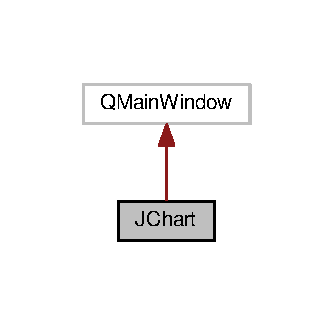
\includegraphics[width=160pt]{class_j_chart__inherit__graph}
\end{center}
\end{figure}


Collaboration diagram for J\+Chart\+:\nopagebreak
\begin{figure}[H]
\begin{center}
\leavevmode
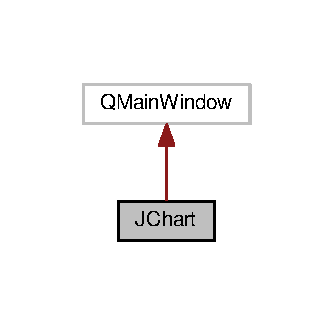
\includegraphics[width=160pt]{class_j_chart__coll__graph}
\end{center}
\end{figure}
\subsection*{Signals}
\begin{DoxyCompactItemize}
\item 
void {\bfseries Signal\+Changed} ()\hypertarget{class_j_chart_ab59324b8e03f64b90c9e414f7ff22a00}{}\label{class_j_chart_ab59324b8e03f64b90c9e414f7ff22a00}

\end{DoxyCompactItemize}
\subsection*{Public Member Functions}
\begin{DoxyCompactItemize}
\item 
{\bfseries J\+Chart} (Q\+Widget $\ast$parent=0)\hypertarget{class_j_chart_a81eedfa59e116cd9b22c10dcb94faa75}{}\label{class_j_chart_a81eedfa59e116cd9b22c10dcb94faa75}

\item 
{\footnotesize template$<$class T $>$ }\\void {\bfseries Plot} (T time\+\_\+series)\hypertarget{class_j_chart_a174b9eaf4c484e352db3ebf7d201e5a3}{}\label{class_j_chart_a174b9eaf4c484e352db3ebf7d201e5a3}

\item 
{\footnotesize template$<$class T $>$ }\\void {\bfseries Plot} (T time\+\_\+series, std\+::string chart\+\_\+title)\hypertarget{class_j_chart_a587dd3656171d836b32c4d3578066e4f}{}\label{class_j_chart_a587dd3656171d836b32c4d3578066e4f}

\end{DoxyCompactItemize}


\subsection{Detailed Description}


Definition at line 29 of file jchart.\+h.


\hypertarget{classjaspl_1_1_j_f_f_t}{}\section{jaspl\+:\+:J\+F\+FT Class Reference}
\label{classjaspl_1_1_j_f_f_t}\index{jaspl\+::\+J\+F\+FT@{jaspl\+::\+J\+F\+FT}}
\subsection*{Public Member Functions}
\begin{DoxyCompactItemize}
\item 
void {\bfseries Setup} (uint size)\hypertarget{classjaspl_1_1_j_f_f_t_a9ae772905c4f41a2de1c8b62683f6b5e}{}\label{classjaspl_1_1_j_f_f_t_a9ae772905c4f41a2de1c8b62683f6b5e}

\item 
{\footnotesize template$<$typename T $>$ }\\void {\bfseries Power\+Spectrum} (T \&input)\hypertarget{classjaspl_1_1_j_f_f_t_a3953d73759cf17cb93f2b1e76691a8fe}{}\label{classjaspl_1_1_j_f_f_t_a3953d73759cf17cb93f2b1e76691a8fe}

\item 
void {\bfseries Tear\+Down} ()\hypertarget{classjaspl_1_1_j_f_f_t_a7ba090708a0e3b6e1dba81574fa52548}{}\label{classjaspl_1_1_j_f_f_t_a7ba090708a0e3b6e1dba81574fa52548}

\end{DoxyCompactItemize}


\subsection{Detailed Description}


Definition at line 15 of file jfft.\+h.


\hypertarget{classjaspl_1_1_j_filter}{}\section{jaspl\+:\+:J\+Filter Class Reference}
\label{classjaspl_1_1_j_filter}\index{jaspl\+::\+J\+Filter@{jaspl\+::\+J\+Filter}}


\subsection{Detailed Description}


Definition at line 21 of file jlinearfilter.\+h.


\hypertarget{classjaspl_1_1j_filter_unit_test}{}\section{jaspl\+:\+:j\+Filter\+Unit\+Test$<$ T $>$ Class Template Reference}
\label{classjaspl_1_1j_filter_unit_test}\index{jaspl\+::j\+Filter\+Unit\+Test$<$ T $>$@{jaspl\+::j\+Filter\+Unit\+Test$<$ T $>$}}
\subsection*{Public Member Functions}
\begin{DoxyCompactItemize}
\item 
void {\bfseries Check\+Filter\+C\+PU} (uint num\+\_\+points)\hypertarget{classjaspl_1_1j_filter_unit_test_ad7d58b5daf92be1e51afacdb3c04419d}{}\label{classjaspl_1_1j_filter_unit_test_ad7d58b5daf92be1e51afacdb3c04419d}

\item 
void {\bfseries Check\+Filter\+G\+PU} (uint num\+\_\+points)\hypertarget{classjaspl_1_1j_filter_unit_test_a875d01230ae647f7615c96065ab41779}{}\label{classjaspl_1_1j_filter_unit_test_a875d01230ae647f7615c96065ab41779}

\end{DoxyCompactItemize}


\subsection{Detailed Description}
\subsubsection*{template$<$typename T$>$\\*
class jaspl\+::j\+Filter\+Unit\+Test$<$ T $>$}



Definition at line 25 of file jfilter\+\_\+unit\+\_\+test.\+h.


\hypertarget{class_j_non_linear_filter}{}\section{J\+Non\+Linear\+Filter Class Reference}
\label{class_j_non_linear_filter}\index{J\+Non\+Linear\+Filter@{J\+Non\+Linear\+Filter}}


\subsection{Detailed Description}


Definition at line 5 of file jnonlinearfilter.\+h.


\hypertarget{classjaspl_1_1_j_vector}{}\section{jaspl\+:\+:J\+Vector$<$ F $>$ Class Template Reference}
\label{classjaspl_1_1_j_vector}\index{jaspl\+::\+J\+Vector$<$ F $>$@{jaspl\+::\+J\+Vector$<$ F $>$}}
\subsection*{Public Member Functions}
\begin{DoxyCompactItemize}
\item 
{\bfseries J\+Vector} (std\+::string raw\+\_\+data)\hypertarget{classjaspl_1_1_j_vector_aec9bccd8f55bdb1977f02fccc7872d86}{}\label{classjaspl_1_1_j_vector_aec9bccd8f55bdb1977f02fccc7872d86}

\item 
{\bfseries J\+Vector} (std\+::vector$<$ F $>$ vec)\hypertarget{classjaspl_1_1_j_vector_ab9a8bee6860dc4ddd3c899b73de93e54}{}\label{classjaspl_1_1_j_vector_ab9a8bee6860dc4ddd3c899b73de93e54}

\item 
{\bfseries J\+Vector} (F $\ast$ptr, uint ptr\+\_\+size)\hypertarget{classjaspl_1_1_j_vector_ae3cee2406660cf6bdd73fd416ca23835}{}\label{classjaspl_1_1_j_vector_ae3cee2406660cf6bdd73fd416ca23835}

\item 
{\bfseries J\+Vector} (uint size)\hypertarget{classjaspl_1_1_j_vector_a91890a543ea9a946a56f616dd9748bcd}{}\label{classjaspl_1_1_j_vector_a91890a543ea9a946a56f616dd9748bcd}

\item 
{\bfseries J\+Vector} (uint size, F fill\+\_\+element)\hypertarget{classjaspl_1_1_j_vector_aea6660117c28bd9a787a3318f3e2c0ec}{}\label{classjaspl_1_1_j_vector_aea6660117c28bd9a787a3318f3e2c0ec}

\item 
\hyperlink{classjaspl_1_1_j_vector}{J\+Vector}$<$ F $>$ {\bfseries operator$\ast$=} (F scalar)\hypertarget{classjaspl_1_1_j_vector_a401ed55d69adaae0850b31082694313f}{}\label{classjaspl_1_1_j_vector_a401ed55d69adaae0850b31082694313f}

\item 
\hyperlink{classjaspl_1_1_j_vector}{J\+Vector}$<$ F $>$ {\bfseries operator$\ast$} (F scalar)\hypertarget{classjaspl_1_1_j_vector_a6e882f97e2c212aebe83817924633099}{}\label{classjaspl_1_1_j_vector_a6e882f97e2c212aebe83817924633099}

\item 
\hyperlink{classjaspl_1_1_j_vector}{J\+Vector}$<$ F $>$ {\bfseries operator+=} (F scalar)\hypertarget{classjaspl_1_1_j_vector_a159125c3544f643484a088391af523c4}{}\label{classjaspl_1_1_j_vector_a159125c3544f643484a088391af523c4}

\item 
void {\bfseries push\+\_\+back} (F element)\hypertarget{classjaspl_1_1_j_vector_a8906043d61595e7737c59706c9ac7643}{}\label{classjaspl_1_1_j_vector_a8906043d61595e7737c59706c9ac7643}

\item 
void {\bfseries push\+\_\+front} (F element)\hypertarget{classjaspl_1_1_j_vector_ada7d072df43b19a445f00fc7e9a36e25}{}\label{classjaspl_1_1_j_vector_ada7d072df43b19a445f00fc7e9a36e25}

\item 
std\+::vector$<$ F $>$\+::iterator {\bfseries begin} ()\hypertarget{classjaspl_1_1_j_vector_ade0638fb564d0c859abdbdc23ba97fa3}{}\label{classjaspl_1_1_j_vector_ade0638fb564d0c859abdbdc23ba97fa3}

\item 
std\+::vector$<$ F $>$\+::iterator {\bfseries end} ()\hypertarget{classjaspl_1_1_j_vector_a47d157a58ee97a0b7170f1cff4f70511}{}\label{classjaspl_1_1_j_vector_a47d157a58ee97a0b7170f1cff4f70511}

\item 
F $\ast$ {\bfseries data} ()\hypertarget{classjaspl_1_1_j_vector_ad52b5a350b0e408a9158cc4c6eba7d0f}{}\label{classjaspl_1_1_j_vector_ad52b5a350b0e408a9158cc4c6eba7d0f}

\item 
F \& {\bfseries operator\mbox{[}$\,$\mbox{]}} (const uint index)\hypertarget{classjaspl_1_1_j_vector_a077310d6ba37aa477e70bfceaa79e916}{}\label{classjaspl_1_1_j_vector_a077310d6ba37aa477e70bfceaa79e916}

\item 
F \& {\bfseries at} (const uint index)\hypertarget{classjaspl_1_1_j_vector_a199548bafdcf1f257368a27ec6243069}{}\label{classjaspl_1_1_j_vector_a199548bafdcf1f257368a27ec6243069}

\item 
void {\bfseries reserve} (uint n)\hypertarget{classjaspl_1_1_j_vector_a4d1ff6d9b08324a8db47087dc5c64efc}{}\label{classjaspl_1_1_j_vector_a4d1ff6d9b08324a8db47087dc5c64efc}

\item 
double {\bfseries norm} ()\hypertarget{classjaspl_1_1_j_vector_a7811d30c896a5411fb8e23d290437f92}{}\label{classjaspl_1_1_j_vector_a7811d30c896a5411fb8e23d290437f92}

\item 
void {\bfseries Normalize} ()\hypertarget{classjaspl_1_1_j_vector_a2144d5df7ed2c44ccd6e43aa586ec484}{}\label{classjaspl_1_1_j_vector_a2144d5df7ed2c44ccd6e43aa586ec484}

\item 
double {\bfseries std\+\_\+dev} ()\hypertarget{classjaspl_1_1_j_vector_a26ad1598c827f28aeb159f036a890c1c}{}\label{classjaspl_1_1_j_vector_a26ad1598c827f28aeb159f036a890c1c}

\item 
double {\bfseries mean} ()\hypertarget{classjaspl_1_1_j_vector_a14a30029d1e440c09f8353b0eb9f8fa0}{}\label{classjaspl_1_1_j_vector_a14a30029d1e440c09f8353b0eb9f8fa0}

\item 
F {\bfseries min} ()\hypertarget{classjaspl_1_1_j_vector_a6bb1cfc7f6c73526cc079a20994abfcd}{}\label{classjaspl_1_1_j_vector_a6bb1cfc7f6c73526cc079a20994abfcd}

\item 
F {\bfseries max} ()\hypertarget{classjaspl_1_1_j_vector_a670b6ae1e2becf0f0c311483ff7ae8b1}{}\label{classjaspl_1_1_j_vector_a670b6ae1e2becf0f0c311483ff7ae8b1}

\item 
uint {\bfseries size} ()\hypertarget{classjaspl_1_1_j_vector_a704189ad3e7f18bc6c2a42df23ce20eb}{}\label{classjaspl_1_1_j_vector_a704189ad3e7f18bc6c2a42df23ce20eb}

\end{DoxyCompactItemize}
\subsection*{Friends}
\begin{DoxyCompactItemize}
\item 
{\footnotesize template$<$class T $>$ }\\void {\bfseries plot} (\hyperlink{classjaspl_1_1_j_vector}{J\+Vector}$<$ T $>$ \&vec)\hypertarget{classjaspl_1_1_j_vector_a6dc51c5dfdd4aacdf08ebad6d0d2afae}{}\label{classjaspl_1_1_j_vector_a6dc51c5dfdd4aacdf08ebad6d0d2afae}

\item 
{\footnotesize template$<$class T $>$ }\\void {\bfseries plot} (\hyperlink{classjaspl_1_1_j_vector}{J\+Vector}$<$ T $>$ \&vec, std\+::string plot\+\_\+title)\hypertarget{classjaspl_1_1_j_vector_a61b154a38160f96e7326fa73252f59ff}{}\label{classjaspl_1_1_j_vector_a61b154a38160f96e7326fa73252f59ff}

\item 
bool {\bfseries operator==} (\hyperlink{classjaspl_1_1_j_vector}{J\+Vector}$<$ F $>$ \&vector\+\_\+a, \hyperlink{classjaspl_1_1_j_vector}{J\+Vector}$<$ F $>$ \&vector\+\_\+b)\hypertarget{classjaspl_1_1_j_vector_a81fad03b34e80d689ede7e6d7178ed56}{}\label{classjaspl_1_1_j_vector_a81fad03b34e80d689ede7e6d7178ed56}

\item 
bool {\bfseries operator!=} (\hyperlink{classjaspl_1_1_j_vector}{J\+Vector}$<$ F $>$ \&vector\+\_\+a, \hyperlink{classjaspl_1_1_j_vector}{J\+Vector}$<$ F $>$ \&vector\+\_\+b)\hypertarget{classjaspl_1_1_j_vector_ad9f0b4638213ca7ffad3c23031a58c35}{}\label{classjaspl_1_1_j_vector_ad9f0b4638213ca7ffad3c23031a58c35}

\item 
std\+::ostream \& {\bfseries operator$<$$<$} (std\+::ostream \&stream, \hyperlink{classjaspl_1_1_j_vector}{J\+Vector}$<$ F $>$ \&spectrum)\hypertarget{classjaspl_1_1_j_vector_a5bb4330c3ad441ee4a22dd90c019f20d}{}\label{classjaspl_1_1_j_vector_a5bb4330c3ad441ee4a22dd90c019f20d}

\item 
std\+::ofstream \& {\bfseries operator$<$$<$} (std\+::ofstream \&stream, \hyperlink{classjaspl_1_1_j_vector}{J\+Vector}$<$ F $>$ \&spectrum)\hypertarget{classjaspl_1_1_j_vector_aa520fbd88b8c88fc26f1d352ac911f37}{}\label{classjaspl_1_1_j_vector_aa520fbd88b8c88fc26f1d352ac911f37}

\item 
\hyperlink{classjaspl_1_1_j_vector}{J\+Vector}$<$ F $>$ {\bfseries operator+} (\hyperlink{classjaspl_1_1_j_vector}{J\+Vector}$<$ F $>$ \&vector\+\_\+a, \hyperlink{classjaspl_1_1_j_vector}{J\+Vector}$<$ F $>$ \&vector\+\_\+b)\hypertarget{classjaspl_1_1_j_vector_ab0c3db97c64f145b82254682de3a9dac}{}\label{classjaspl_1_1_j_vector_ab0c3db97c64f145b82254682de3a9dac}

\item 
\hyperlink{classjaspl_1_1_j_vector}{J\+Vector}$<$ F $>$ {\bfseries operator+} (\hyperlink{classjaspl_1_1_j_vector}{J\+Vector}$<$ F $>$ \&vector\+\_\+a, std\+::vector$<$ F $>$ \&vector\+\_\+b)\hypertarget{classjaspl_1_1_j_vector_a2d32b7256486f2427723aa03d2e21016}{}\label{classjaspl_1_1_j_vector_a2d32b7256486f2427723aa03d2e21016}

\item 
\hyperlink{classjaspl_1_1_j_vector}{J\+Vector}$<$ F $>$ {\bfseries operator-\/} (\hyperlink{classjaspl_1_1_j_vector}{J\+Vector}$<$ F $>$ \&vector\+\_\+a, \hyperlink{classjaspl_1_1_j_vector}{J\+Vector}$<$ F $>$ \&vector\+\_\+b)\hypertarget{classjaspl_1_1_j_vector_a0346f9409f8dbf1c202a587bd4be6e6d}{}\label{classjaspl_1_1_j_vector_a0346f9409f8dbf1c202a587bd4be6e6d}

\item 
\hyperlink{classjaspl_1_1_j_vector}{J\+Vector}$<$ F $>$ {\bfseries operator-\/} (\hyperlink{classjaspl_1_1_j_vector}{J\+Vector}$<$ F $>$ \&vector\+\_\+a, std\+::vector$<$ F $>$ \&vector\+\_\+b)\hypertarget{classjaspl_1_1_j_vector_ae6badaa441ef27ab6140d8dcec31eae8}{}\label{classjaspl_1_1_j_vector_ae6badaa441ef27ab6140d8dcec31eae8}

\item 
\hyperlink{classjaspl_1_1_j_vector}{J\+Vector}$<$ F $>$ {\bfseries operator$\ast$} (\hyperlink{classjaspl_1_1_j_vector}{J\+Vector}$<$ F $>$ \&vector\+\_\+a, \hyperlink{classjaspl_1_1_j_vector}{J\+Vector}$<$ F $>$ \&vector\+\_\+b)\hypertarget{classjaspl_1_1_j_vector_a2c5ea5529b0e58fd7cca8431b618d909}{}\label{classjaspl_1_1_j_vector_a2c5ea5529b0e58fd7cca8431b618d909}

\item 
\hyperlink{classjaspl_1_1_j_vector}{J\+Vector}$<$ F $>$ {\bfseries operator$\ast$} (\hyperlink{classjaspl_1_1_j_vector}{J\+Vector}$<$ F $>$ \&vector\+\_\+a, std\+::vector$<$ F $>$ \&vector\+\_\+b)\hypertarget{classjaspl_1_1_j_vector_a357e9f8d65a0e055329173fc96a269dc}{}\label{classjaspl_1_1_j_vector_a357e9f8d65a0e055329173fc96a269dc}

\end{DoxyCompactItemize}


\subsection{Detailed Description}
\subsubsection*{template$<$class F$>$\\*
class jaspl\+::\+J\+Vector$<$ F $>$}



Definition at line 20 of file jvector.\+h.


\hypertarget{classjaspl_1_1ocl_1_1_linear_convolution}{}\section{jaspl\+:\+:ocl\+:\+:Linear\+Convolution$<$ T $>$ Class Template Reference}
\label{classjaspl_1_1ocl_1_1_linear_convolution}\index{jaspl\+::ocl\+::\+Linear\+Convolution$<$ T $>$@{jaspl\+::ocl\+::\+Linear\+Convolution$<$ T $>$}}


Inheritance diagram for jaspl\+:\+:ocl\+:\+:Linear\+Convolution$<$ T $>$\+:\nopagebreak
\begin{figure}[H]
\begin{center}
\leavevmode
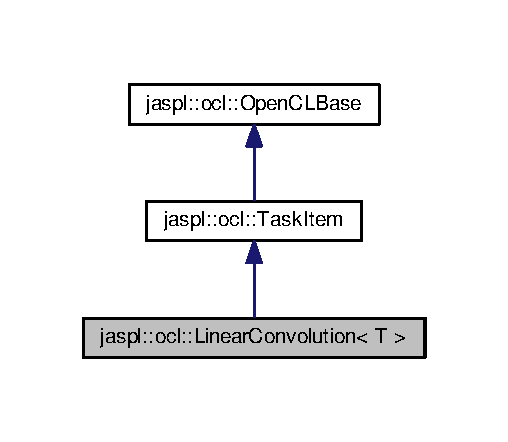
\includegraphics[width=244pt]{classjaspl_1_1ocl_1_1_linear_convolution__inherit__graph}
\end{center}
\end{figure}


Collaboration diagram for jaspl\+:\+:ocl\+:\+:Linear\+Convolution$<$ T $>$\+:\nopagebreak
\begin{figure}[H]
\begin{center}
\leavevmode
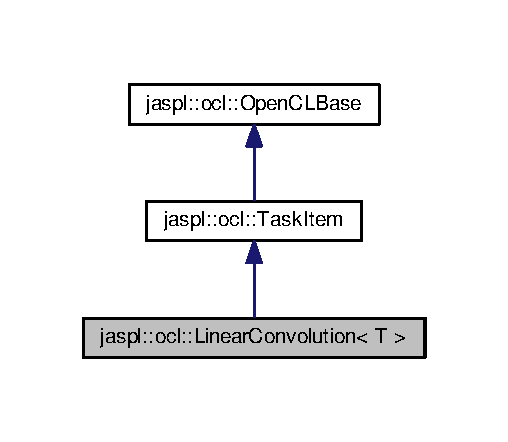
\includegraphics[width=244pt]{classjaspl_1_1ocl_1_1_linear_convolution__coll__graph}
\end{center}
\end{figure}
\subsection*{Public Member Functions}
\begin{DoxyCompactItemize}
\item 
{\bfseries Linear\+Convolution} (T \&convolution\+\_\+kernel)\hypertarget{classjaspl_1_1ocl_1_1_linear_convolution_ace2eaebe26dc0cd81332da88ecb686dd}{}\label{classjaspl_1_1ocl_1_1_linear_convolution_ace2eaebe26dc0cd81332da88ecb686dd}

\item 
{\bfseries Linear\+Convolution} (T $\ast$convolution\+\_\+kernel)\hypertarget{classjaspl_1_1ocl_1_1_linear_convolution_a24010f98b35669374fd0ac03e70a4ee2}{}\label{classjaspl_1_1ocl_1_1_linear_convolution_a24010f98b35669374fd0ac03e70a4ee2}

\end{DoxyCompactItemize}
\subsection*{Additional Inherited Members}


\subsection{Detailed Description}
\subsubsection*{template$<$class T$>$\\*
class jaspl\+::ocl\+::\+Linear\+Convolution$<$ T $>$}



Definition at line 23 of file linearconvolution.\+h.


\hypertarget{classjaspl_1_1ocl_1_1_non_linear_convolution}{}\section{jaspl\+:\+:ocl\+:\+:Non\+Linear\+Convolution$<$ T $>$ Class Template Reference}
\label{classjaspl_1_1ocl_1_1_non_linear_convolution}\index{jaspl\+::ocl\+::\+Non\+Linear\+Convolution$<$ T $>$@{jaspl\+::ocl\+::\+Non\+Linear\+Convolution$<$ T $>$}}


Inheritance diagram for jaspl\+:\+:ocl\+:\+:Non\+Linear\+Convolution$<$ T $>$\+:\nopagebreak
\begin{figure}[H]
\begin{center}
\leavevmode
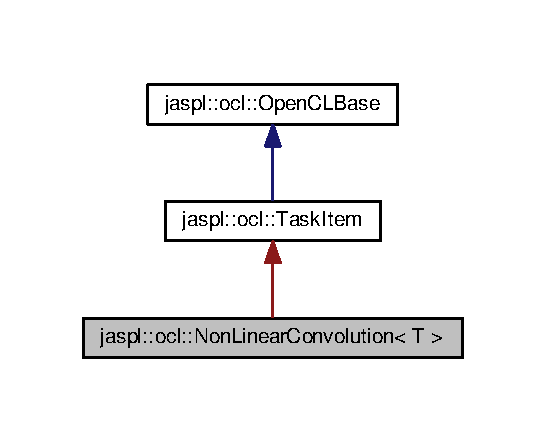
\includegraphics[width=262pt]{classjaspl_1_1ocl_1_1_non_linear_convolution__inherit__graph}
\end{center}
\end{figure}


Collaboration diagram for jaspl\+:\+:ocl\+:\+:Non\+Linear\+Convolution$<$ T $>$\+:\nopagebreak
\begin{figure}[H]
\begin{center}
\leavevmode
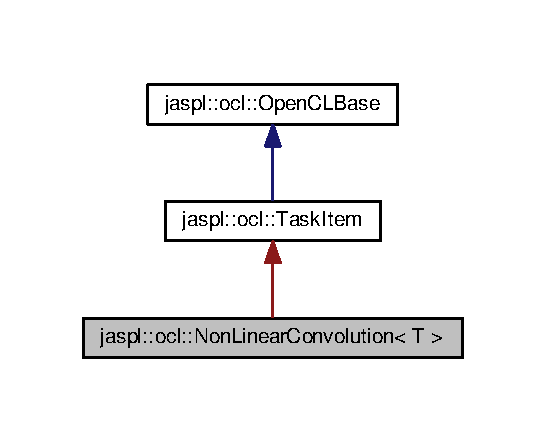
\includegraphics[width=262pt]{classjaspl_1_1ocl_1_1_non_linear_convolution__coll__graph}
\end{center}
\end{figure}
\subsection*{Public Member Functions}
\begin{DoxyCompactItemize}
\item 
{\bfseries Non\+Linear\+Convolution} (T \&convolution\+\_\+kernel)\hypertarget{classjaspl_1_1ocl_1_1_non_linear_convolution_a85fb33c4e6d02633ca25df3d3d659a3c}{}\label{classjaspl_1_1ocl_1_1_non_linear_convolution_a85fb33c4e6d02633ca25df3d3d659a3c}

\item 
{\bfseries Non\+Linear\+Convolution} (T $\ast$convolution\+\_\+kernel)\hypertarget{classjaspl_1_1ocl_1_1_non_linear_convolution_a05dfb729106ccc73d7e1d31ba5b98694}{}\label{classjaspl_1_1ocl_1_1_non_linear_convolution_a05dfb729106ccc73d7e1d31ba5b98694}

\end{DoxyCompactItemize}


\subsection{Detailed Description}
\subsubsection*{template$<$class T$>$\\*
class jaspl\+::ocl\+::\+Non\+Linear\+Convolution$<$ T $>$}



Definition at line 23 of file nonlinearconvolution.\+h.


\hypertarget{classjaspl_1_1ocl_1_1_open_c_l_base}{}\section{jaspl\+:\+:ocl\+:\+:Open\+C\+L\+Base Class Reference}
\label{classjaspl_1_1ocl_1_1_open_c_l_base}\index{jaspl\+::ocl\+::\+Open\+C\+L\+Base@{jaspl\+::ocl\+::\+Open\+C\+L\+Base}}


Base class for every class that needs access to Open\+CL Platforms, Contexts or Devices.  




{\ttfamily \#include $<$openclbase.\+h$>$}



Inheritance diagram for jaspl\+:\+:ocl\+:\+:Open\+C\+L\+Base\+:
\nopagebreak
\begin{figure}[H]
\begin{center}
\leavevmode
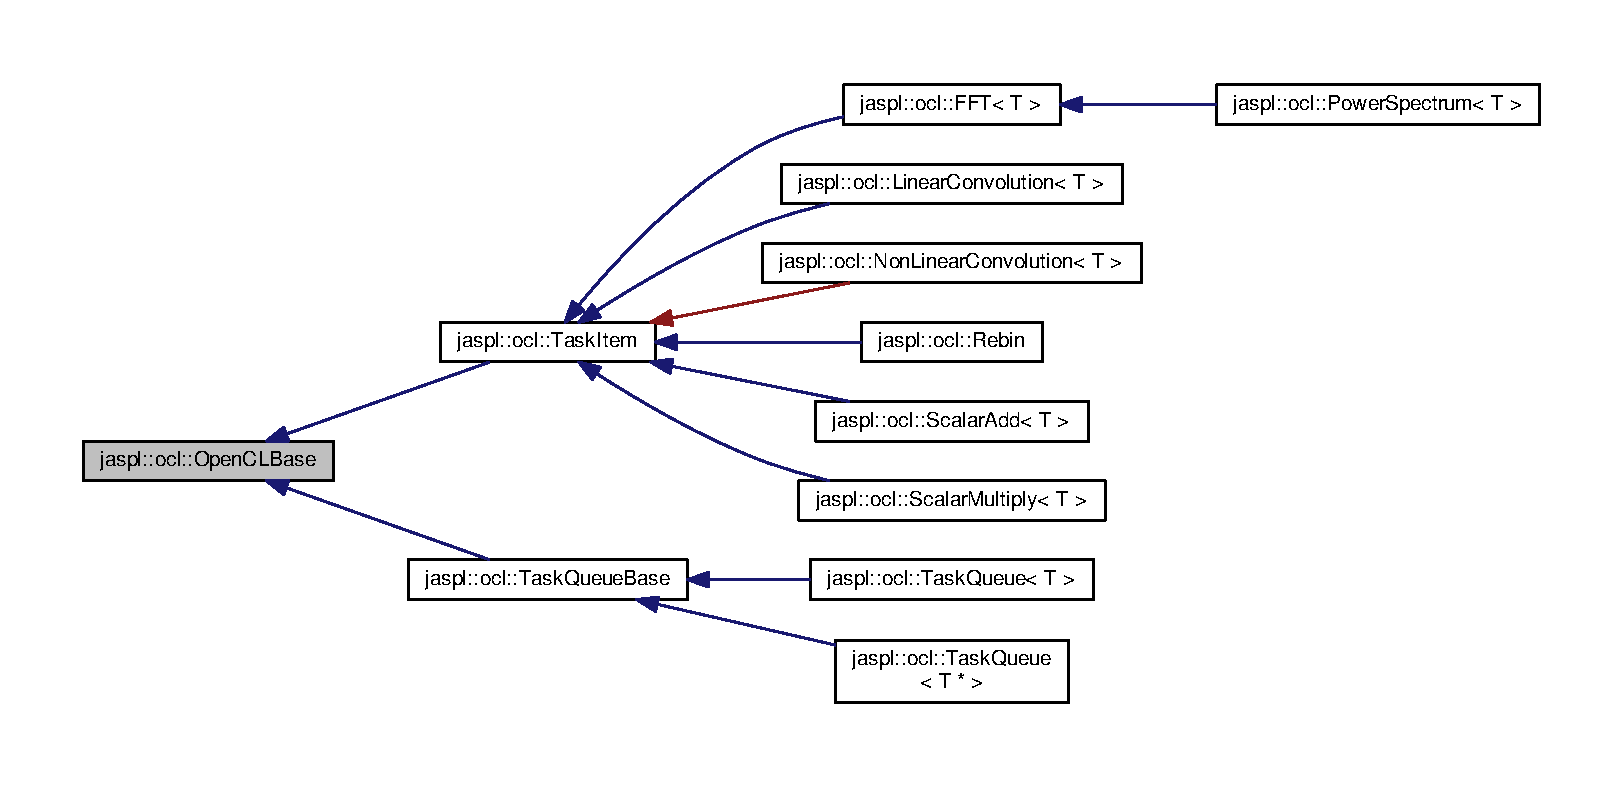
\includegraphics[width=350pt]{classjaspl_1_1ocl_1_1_open_c_l_base__inherit__graph}
\end{center}
\end{figure}
\subsection*{Public Member Functions}
\begin{DoxyCompactItemize}
\item 
\hyperlink{classjaspl_1_1ocl_1_1_open_c_l_base_a60c09a482b92e3e5fcaa488fcd391dcb}{Open\+C\+L\+Base} (uint platform\+\_\+number=0, uint device\+\_\+number=0)
\begin{DoxyCompactList}\small\item\em Initialize Open\+CL Objects Note that the Platform and Context are selected automatically\+: Platform is set to cl\+::\+Platform( 0 ) Context is set to cl\+::\+Context( device\mbox{[} device\+\_\+number \mbox{]} ) \end{DoxyCompactList}\end{DoxyCompactItemize}
\subsection*{Protected Member Functions}
\begin{DoxyCompactItemize}
\item 
void {\bfseries Set\+Up} (uint platform\+\_\+number, uint device\+\_\+number)\hypertarget{classjaspl_1_1ocl_1_1_open_c_l_base_a18031bd6b0e52aefeff4b28e98fcda96}{}\label{classjaspl_1_1ocl_1_1_open_c_l_base_a18031bd6b0e52aefeff4b28e98fcda96}

\end{DoxyCompactItemize}
\subsection*{Static Protected Attributes}
\begin{DoxyCompactItemize}
\item 
static bool {\bfseries initalized} = false\hypertarget{classjaspl_1_1ocl_1_1_open_c_l_base_ad8942a3114b511028404945d2b658689}{}\label{classjaspl_1_1ocl_1_1_open_c_l_base_ad8942a3114b511028404945d2b658689}

\item 
static std\+::vector$<$ cl\+::\+Platform $>$ {\bfseries all\+\_\+platforms}\hypertarget{classjaspl_1_1ocl_1_1_open_c_l_base_aca4e1b8a9db57208f0f4aa93053551c5}{}\label{classjaspl_1_1ocl_1_1_open_c_l_base_aca4e1b8a9db57208f0f4aa93053551c5}

\item 
static cl\+::\+Platform {\bfseries default\+\_\+platform}\hypertarget{classjaspl_1_1ocl_1_1_open_c_l_base_adba19ace68e13d2aef858d62be78305d}{}\label{classjaspl_1_1ocl_1_1_open_c_l_base_adba19ace68e13d2aef858d62be78305d}

\item 
static std\+::vector$<$ cl\+::\+Device $>$ {\bfseries all\+\_\+devices}\hypertarget{classjaspl_1_1ocl_1_1_open_c_l_base_a38970dc6296c7e86cbd2e53ed96dbf89}{}\label{classjaspl_1_1ocl_1_1_open_c_l_base_a38970dc6296c7e86cbd2e53ed96dbf89}

\item 
static cl\+::\+Device {\bfseries current\+\_\+device}\hypertarget{classjaspl_1_1ocl_1_1_open_c_l_base_ab98895e065dcdbb77e82d68fe50f3656}{}\label{classjaspl_1_1ocl_1_1_open_c_l_base_ab98895e065dcdbb77e82d68fe50f3656}

\item 
static cl\+::\+Context {\bfseries context}\hypertarget{classjaspl_1_1ocl_1_1_open_c_l_base_a630838c8c08a6bda110e04c2dda66850}{}\label{classjaspl_1_1ocl_1_1_open_c_l_base_a630838c8c08a6bda110e04c2dda66850}

\item 
static cl\+::\+Command\+Queue {\bfseries command\+\_\+queue}\hypertarget{classjaspl_1_1ocl_1_1_open_c_l_base_a96aae0bed8da50e336194b437c159e4a}{}\label{classjaspl_1_1ocl_1_1_open_c_l_base_a96aae0bed8da50e336194b437c159e4a}

\end{DoxyCompactItemize}


\subsection{Detailed Description}
Base class for every class that needs access to Open\+CL Platforms, Contexts or Devices. 

This class a common Open\+CL Platform, Context, Command\+Queue and Device for derived classes to share. 

Definition at line 31 of file openclbase.\+h.



\subsection{Constructor \& Destructor Documentation}
\index{jaspl\+::ocl\+::\+Open\+C\+L\+Base@{jaspl\+::ocl\+::\+Open\+C\+L\+Base}!Open\+C\+L\+Base@{Open\+C\+L\+Base}}
\index{Open\+C\+L\+Base@{Open\+C\+L\+Base}!jaspl\+::ocl\+::\+Open\+C\+L\+Base@{jaspl\+::ocl\+::\+Open\+C\+L\+Base}}
\subsubsection[{\texorpdfstring{Open\+C\+L\+Base(uint platform\+\_\+number=0, uint device\+\_\+number=0)}{OpenCLBase(uint platform_number=0, uint device_number=0)}}]{\setlength{\rightskip}{0pt plus 5cm}jaspl\+::ocl\+::\+Open\+C\+L\+Base\+::\+Open\+C\+L\+Base (
\begin{DoxyParamCaption}
\item[{uint}]{platform\+\_\+number = {\ttfamily 0}, }
\item[{uint}]{device\+\_\+number = {\ttfamily 0}}
\end{DoxyParamCaption}
)}\hypertarget{classjaspl_1_1ocl_1_1_open_c_l_base_a60c09a482b92e3e5fcaa488fcd391dcb}{}\label{classjaspl_1_1ocl_1_1_open_c_l_base_a60c09a482b92e3e5fcaa488fcd391dcb}


Initialize Open\+CL Objects Note that the Platform and Context are selected automatically\+: Platform is set to cl\+::\+Platform( 0 ) Context is set to cl\+::\+Context( device\mbox{[} device\+\_\+number \mbox{]} ) 

The underlying assumption is that the host machine has only one Open\+CL Platform ( e.\+g. one of A\+M\+D-\/\+A\+PP, Nvidia C\+U\+DA, Intel )


\begin{DoxyParams}{Parameters}
{\em device\+\_\+number} & Number of the Open\+CL device to use as described by cl\+::\+Platform\+::get\+Devices(\+C\+L\+\_\+\+D\+E\+V\+I\+C\+E\+\_\+\+T\+Y\+P\+E\+\_\+\+A\+L\+L) \\
\hline
\end{DoxyParams}


Definition at line 78 of file openclbase.\+cpp.


\hypertarget{classjaspl_1_1ouroborus}{}\section{jaspl\+:\+:ouroborus$<$ T $>$ Class Template Reference}
\label{classjaspl_1_1ouroborus}\index{jaspl\+::ouroborus$<$ T $>$@{jaspl\+::ouroborus$<$ T $>$}}
\subsection*{Public Member Functions}
\begin{DoxyCompactItemize}
\item 
{\bfseries ouroborus} (uint buffer\+\_\+size)\hypertarget{classjaspl_1_1ouroborus_afc5380d2850dd026af3c3d70d150bf60}{}\label{classjaspl_1_1ouroborus_afc5380d2850dd026af3c3d70d150bf60}

\item 
void {\bfseries Head\+Insert} (T $\ast$to\+\_\+insert, uint insert\+\_\+size)\hypertarget{classjaspl_1_1ouroborus_a6d16f36785bb75315e520fcb17f46b8c}{}\label{classjaspl_1_1ouroborus_a6d16f36785bb75315e520fcb17f46b8c}

\item 
void {\bfseries Tail\+Insert} (T $\ast$to\+\_\+insert, uint insert\+\_\+size)\hypertarget{classjaspl_1_1ouroborus_a7592cd37c22235d01d306d36ca8da370}{}\label{classjaspl_1_1ouroborus_a7592cd37c22235d01d306d36ca8da370}

\item 
std\+::vector$<$ T $>$ {\bfseries Head\+Read} (uint read\+\_\+size)\hypertarget{classjaspl_1_1ouroborus_a4bc7a38915ec1bebfcc185b0d626ba19}{}\label{classjaspl_1_1ouroborus_a4bc7a38915ec1bebfcc185b0d626ba19}

\item 
{\footnotesize template$<$typename F $>$ }\\std\+::vector$<$ F $>$ {\bfseries Head\+Read\+And\+Convert} (uint read\+\_\+size)\hypertarget{classjaspl_1_1ouroborus_a3927bb1e83d608b0c0ef8a2f50a17b9d}{}\label{classjaspl_1_1ouroborus_a3927bb1e83d608b0c0ef8a2f50a17b9d}

\item 
bool {\bfseries Check\+Head} (uint read\+\_\+size)\hypertarget{classjaspl_1_1ouroborus_ac595602b6e133b4c6cef5ffed2ff1fbd}{}\label{classjaspl_1_1ouroborus_ac595602b6e133b4c6cef5ffed2ff1fbd}

\item 
std\+::vector$<$ T $>$ {\bfseries Tail\+Read} (uint read\+\_\+size)\hypertarget{classjaspl_1_1ouroborus_a81fe174d4952d7e0eb5e2008d0971bae}{}\label{classjaspl_1_1ouroborus_a81fe174d4952d7e0eb5e2008d0971bae}

\item 
{\footnotesize template$<$typename F $>$ }\\std\+::vector$<$ F $>$ {\bfseries Tail\+Read\+And\+Convert} (uint read\+\_\+size)\hypertarget{classjaspl_1_1ouroborus_aec03e5659e53b7f47b011ae8f4ed005d}{}\label{classjaspl_1_1ouroborus_aec03e5659e53b7f47b011ae8f4ed005d}

\item 
bool {\bfseries Check\+Tail} (uint read\+\_\+size)\hypertarget{classjaspl_1_1ouroborus_ac22cf95482e411c2197aed495c97d8e6}{}\label{classjaspl_1_1ouroborus_ac22cf95482e411c2197aed495c97d8e6}

\item 
void {\bfseries Reset} ()\hypertarget{classjaspl_1_1ouroborus_a5310f41f32ed0961a4658752066e8cca}{}\label{classjaspl_1_1ouroborus_a5310f41f32ed0961a4658752066e8cca}

\item 
uint {\bfseries capacity} ()\hypertarget{classjaspl_1_1ouroborus_a212abb4f554e9bb68d6570a9215b6896}{}\label{classjaspl_1_1ouroborus_a212abb4f554e9bb68d6570a9215b6896}

\item 
uint {\bfseries size} ()\hypertarget{classjaspl_1_1ouroborus_a417ccee8ba98c637c569c45f466bfa21}{}\label{classjaspl_1_1ouroborus_a417ccee8ba98c637c569c45f466bfa21}

\item 
bool {\bfseries overrun} ()\hypertarget{classjaspl_1_1ouroborus_a83fca643268f7cc436833e82b557bcea}{}\label{classjaspl_1_1ouroborus_a83fca643268f7cc436833e82b557bcea}

\end{DoxyCompactItemize}
\subsection*{Friends}
\begin{DoxyCompactItemize}
\item 
{\footnotesize template$<$typename F $>$ }\\std\+::ostream \& {\bfseries operator$<$$<$} (std\+::ostream \&stream, \hyperlink{classjaspl_1_1ouroborus}{ouroborus}$<$ F $>$ \&buffer)\hypertarget{classjaspl_1_1ouroborus_a0c1f627811212d72eb869d0bf3db05ec}{}\label{classjaspl_1_1ouroborus_a0c1f627811212d72eb869d0bf3db05ec}

\end{DoxyCompactItemize}


\subsection{Detailed Description}
\subsubsection*{template$<$typename T$>$\\*
class jaspl\+::ouroborus$<$ T $>$}



Definition at line 22 of file ouroboros.\+h.


\hypertarget{classjaspl_1_1_plotter}{}\section{jaspl\+:\+:Plotter$<$ T $>$ Class Template Reference}
\label{classjaspl_1_1_plotter}\index{jaspl\+::\+Plotter$<$ T $>$@{jaspl\+::\+Plotter$<$ T $>$}}
\subsection*{Public Member Functions}
\begin{DoxyCompactItemize}
\item 
void {\bfseries Plot} ()\hypertarget{classjaspl_1_1_plotter_a2bf19310ad5f950c5779a7a94738a186}{}\label{classjaspl_1_1_plotter_a2bf19310ad5f950c5779a7a94738a186}

\item 
void {\bfseries Set\+X\+Axis\+Label} (std\+::string x\+\_\+label)\hypertarget{classjaspl_1_1_plotter_ac456827d783af794673e18d24758512b}{}\label{classjaspl_1_1_plotter_ac456827d783af794673e18d24758512b}

\item 
void {\bfseries Set\+Y\+Axis\+Label} (std\+::string y\+\_\+label)\hypertarget{classjaspl_1_1_plotter_af2fe690d3e8dd14374ef67de010c60f2}{}\label{classjaspl_1_1_plotter_af2fe690d3e8dd14374ef67de010c60f2}

\item 
void {\bfseries Set\+Save\+Path} (std\+::string file\+\_\+path)\hypertarget{classjaspl_1_1_plotter_a68f0532d49ea6673ff4ae666f95dc5d9}{}\label{classjaspl_1_1_plotter_a68f0532d49ea6673ff4ae666f95dc5d9}

\item 
void {\bfseries Add\+Series} (T series, std\+::string title)\hypertarget{classjaspl_1_1_plotter_a61783f71df3253ed393d16ba98b304c2}{}\label{classjaspl_1_1_plotter_a61783f71df3253ed393d16ba98b304c2}

\item 
void {\bfseries Set\+Max\+Num\+Points} (uint max\+\_\+points)\hypertarget{classjaspl_1_1_plotter_a382677a28083b7bd1a86f045ae721424}{}\label{classjaspl_1_1_plotter_a382677a28083b7bd1a86f045ae721424}

\end{DoxyCompactItemize}


\subsection{Detailed Description}
\subsubsection*{template$<$typename T$>$\\*
class jaspl\+::\+Plotter$<$ T $>$}



Definition at line 20 of file jplot.\+h.


\hypertarget{classjaspl_1_1ocl_1_1_power_spectrum}{}\section{jaspl\+:\+:ocl\+:\+:Power\+Spectrum$<$ T $>$ Class Template Reference}
\label{classjaspl_1_1ocl_1_1_power_spectrum}\index{jaspl\+::ocl\+::\+Power\+Spectrum$<$ T $>$@{jaspl\+::ocl\+::\+Power\+Spectrum$<$ T $>$}}


Inheritance diagram for jaspl\+:\+:ocl\+:\+:Power\+Spectrum$<$ T $>$\+:\nopagebreak
\begin{figure}[H]
\begin{center}
\leavevmode
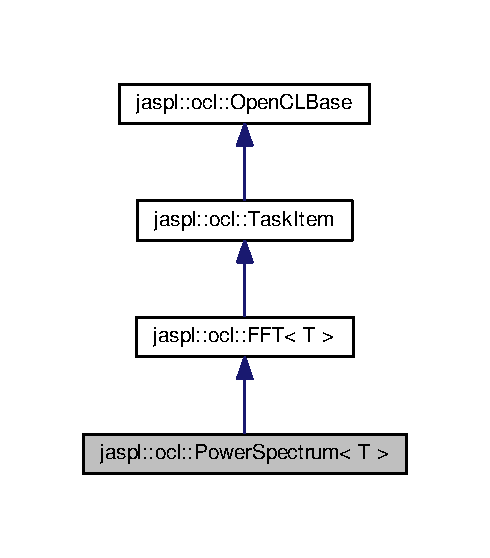
\includegraphics[width=235pt]{classjaspl_1_1ocl_1_1_power_spectrum__inherit__graph}
\end{center}
\end{figure}


Collaboration diagram for jaspl\+:\+:ocl\+:\+:Power\+Spectrum$<$ T $>$\+:\nopagebreak
\begin{figure}[H]
\begin{center}
\leavevmode
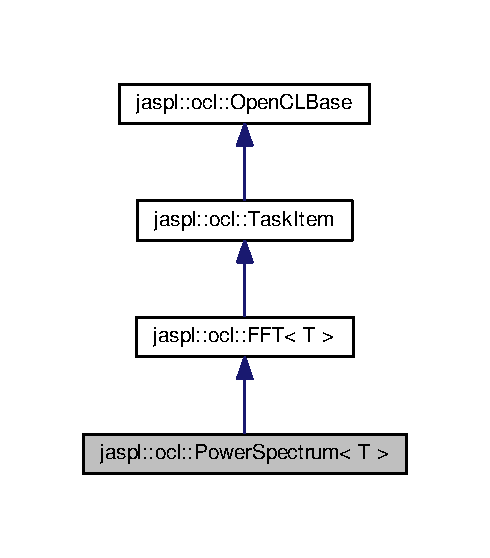
\includegraphics[width=235pt]{classjaspl_1_1ocl_1_1_power_spectrum__coll__graph}
\end{center}
\end{figure}
\subsection*{Additional Inherited Members}


\subsection{Detailed Description}
\subsubsection*{template$<$class T$>$\\*
class jaspl\+::ocl\+::\+Power\+Spectrum$<$ T $>$}



Definition at line 23 of file powerspectrum.\+h.


\hypertarget{classjaspl_1_1ocl_1_1_rebin}{}\section{jaspl\+:\+:ocl\+:\+:Rebin Class Reference}
\label{classjaspl_1_1ocl_1_1_rebin}\index{jaspl\+::ocl\+::\+Rebin@{jaspl\+::ocl\+::\+Rebin}}


Inheritance diagram for jaspl\+:\+:ocl\+:\+:Rebin\+:\nopagebreak
\begin{figure}[H]
\begin{center}
\leavevmode
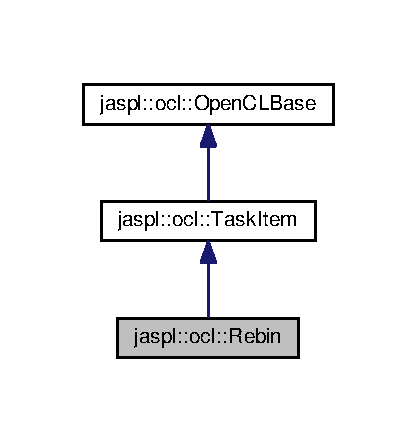
\includegraphics[width=200pt]{classjaspl_1_1ocl_1_1_rebin__inherit__graph}
\end{center}
\end{figure}


Collaboration diagram for jaspl\+:\+:ocl\+:\+:Rebin\+:\nopagebreak
\begin{figure}[H]
\begin{center}
\leavevmode
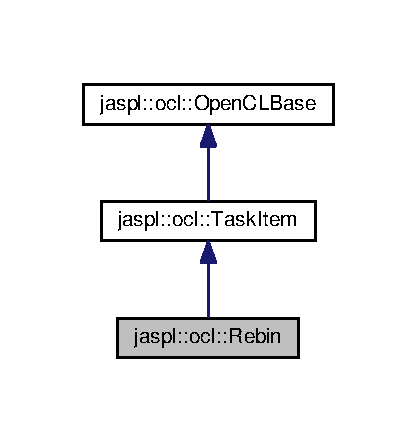
\includegraphics[width=200pt]{classjaspl_1_1ocl_1_1_rebin__coll__graph}
\end{center}
\end{figure}
\subsection*{Additional Inherited Members}


\subsection{Detailed Description}


Definition at line 21 of file rebin.\+h.


\hypertarget{classjaspl_1_1_recurse_mean}{}\section{jaspl\+:\+:Recurse\+Mean$<$ T $>$ Class Template Reference}
\label{classjaspl_1_1_recurse_mean}\index{jaspl\+::\+Recurse\+Mean$<$ T $>$@{jaspl\+::\+Recurse\+Mean$<$ T $>$}}


Average together a (nearly) arbitrary number of container-\/like objects using the recursive definition of the expected value defined by\+:  




{\ttfamily \#include $<$jalgorithm.\+h$>$}

\subsection*{Public Member Functions}
\begin{DoxyCompactItemize}
\item 
{\bfseries Recurse\+Mean} (uint num\+\_\+samples)\hypertarget{classjaspl_1_1_recurse_mean_abbcaa2624b48de1a68407cc44ca9068d}{}\label{classjaspl_1_1_recurse_mean_abbcaa2624b48de1a68407cc44ca9068d}

\item 
void \hyperlink{classjaspl_1_1_recurse_mean_a5c65990ad47245fcf866ad811cd340c3}{operator()} (const T \&next\+\_\+value)
\begin{DoxyCompactList}\small\item\em Average together a new value. \end{DoxyCompactList}\item 
void {\bfseries Reset} ()\hypertarget{classjaspl_1_1_recurse_mean_ac661dff7908c06fe1701feb7d0d07af5}{}\label{classjaspl_1_1_recurse_mean_ac661dff7908c06fe1701feb7d0d07af5}

\item 
T {\bfseries Return\+Value} ()\hypertarget{classjaspl_1_1_recurse_mean_ad9ec10f40cbfdc5f9799be43e0855572}{}\label{classjaspl_1_1_recurse_mean_ad9ec10f40cbfdc5f9799be43e0855572}

\end{DoxyCompactItemize}


\subsection{Detailed Description}
\subsubsection*{template$<$typename T$>$\\*
class jaspl\+::\+Recurse\+Mean$<$ T $>$}

Average together a (nearly) arbitrary number of container-\/like objects using the recursive definition of the expected value defined by\+: 

\[ \mu_i = \frac{ i - 1 }{ i } \mu_{ i - 1 } + \frac{1}{i} x_i\\ \text{ for } x_i \in \mathbb{R}^n \ \mu_i \in \mathcal{R} \\ \text{ and running index } i \in \mathbb{N} \]

Template parameter needs to be a container-\/liker object filled with floating-\/point values. 

Definition at line 33 of file jalgorithm.\+h.



\subsection{Member Function Documentation}
\index{jaspl\+::\+Recurse\+Mean@{jaspl\+::\+Recurse\+Mean}!operator()@{operator()}}
\index{operator()@{operator()}!jaspl\+::\+Recurse\+Mean@{jaspl\+::\+Recurse\+Mean}}
\subsubsection[{\texorpdfstring{operator()(const T \&next\+\_\+value)}{operator()(const T &next_value)}}]{\setlength{\rightskip}{0pt plus 5cm}template$<$typename T $>$ void {\bf jaspl\+::\+Recurse\+Mean}$<$ T $>$\+::operator() (
\begin{DoxyParamCaption}
\item[{const T \&}]{next\+\_\+value}
\end{DoxyParamCaption}
)}\hypertarget{classjaspl_1_1_recurse_mean_a5c65990ad47245fcf866ad811cd340c3}{}\label{classjaspl_1_1_recurse_mean_a5c65990ad47245fcf866ad811cd340c3}


Average together a new value. 


\begin{DoxyParams}{Parameters}
{\em next\+\_\+value} & The container to be averaged \\
\hline
\end{DoxyParams}

\hypertarget{classjaspl_1_1ocl_1_1_scalar_add}{}\section{jaspl\+:\+:ocl\+:\+:Scalar\+Add$<$ T $>$ Class Template Reference}
\label{classjaspl_1_1ocl_1_1_scalar_add}\index{jaspl\+::ocl\+::\+Scalar\+Add$<$ T $>$@{jaspl\+::ocl\+::\+Scalar\+Add$<$ T $>$}}


Inheritance diagram for jaspl\+:\+:ocl\+:\+:Scalar\+Add$<$ T $>$\+:\nopagebreak
\begin{figure}[H]
\begin{center}
\leavevmode
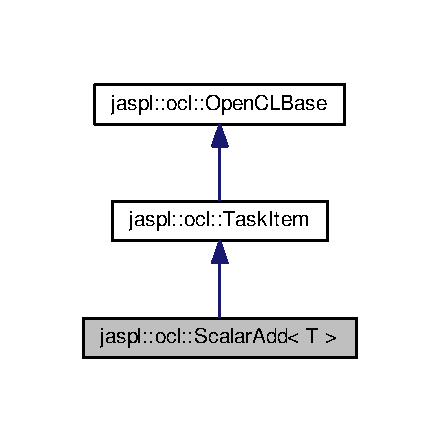
\includegraphics[width=211pt]{classjaspl_1_1ocl_1_1_scalar_add__inherit__graph}
\end{center}
\end{figure}


Collaboration diagram for jaspl\+:\+:ocl\+:\+:Scalar\+Add$<$ T $>$\+:\nopagebreak
\begin{figure}[H]
\begin{center}
\leavevmode
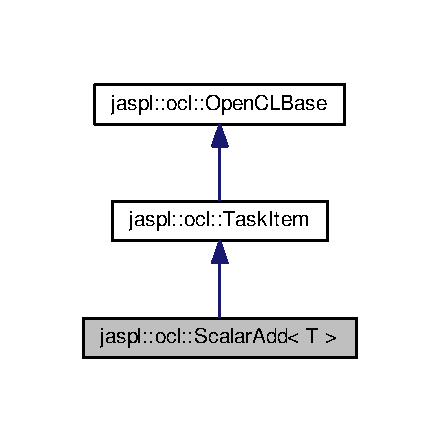
\includegraphics[width=211pt]{classjaspl_1_1ocl_1_1_scalar_add__coll__graph}
\end{center}
\end{figure}
\subsection*{Public Member Functions}
\begin{DoxyCompactItemize}
\item 
{\bfseries Scalar\+Add} (typename T\+::value\+\_\+type scalar\+\_\+value)\hypertarget{classjaspl_1_1ocl_1_1_scalar_add_a74c7684b1023fb5505afa57b65bbee2f}{}\label{classjaspl_1_1ocl_1_1_scalar_add_a74c7684b1023fb5505afa57b65bbee2f}

\end{DoxyCompactItemize}
\subsection*{Protected Member Functions}
\begin{DoxyCompactItemize}
\item 
void {\bfseries Trigger} ()\hypertarget{classjaspl_1_1ocl_1_1_scalar_add_a06f80054324b32d2a396f44e4220b061}{}\label{classjaspl_1_1ocl_1_1_scalar_add_a06f80054324b32d2a396f44e4220b061}

\item 
void {\bfseries Set\+Signal} (cl\+::\+Buffer \&signal\+\_\+buff, uint sig\+\_\+size)\hypertarget{classjaspl_1_1ocl_1_1_scalar_add_a5bb316f923cc37d6dff1144c1832decd}{}\label{classjaspl_1_1ocl_1_1_scalar_add_a5bb316f923cc37d6dff1144c1832decd}

\item 
cl\+::\+Buffer \& {\bfseries Processed\+Signal} ()\hypertarget{classjaspl_1_1ocl_1_1_scalar_add_a11727ab5b2e2c8bf8bdb8c9b8301caa0}{}\label{classjaspl_1_1ocl_1_1_scalar_add_a11727ab5b2e2c8bf8bdb8c9b8301caa0}

\item 
size\+\_\+t {\bfseries Processed\+Signal\+Bytes} ()\hypertarget{classjaspl_1_1ocl_1_1_scalar_add_aab31c814169b8419da653a79a150e3d2}{}\label{classjaspl_1_1ocl_1_1_scalar_add_aab31c814169b8419da653a79a150e3d2}

\item 
size\+\_\+t {\bfseries Processed\+Signal\+Size} ()\hypertarget{classjaspl_1_1ocl_1_1_scalar_add_a1af2d6e8f8ccf876f80afa76b9d47205}{}\label{classjaspl_1_1ocl_1_1_scalar_add_a1af2d6e8f8ccf876f80afa76b9d47205}

\item 
bool {\bfseries Needs\+To\+Reknew} ()\hypertarget{classjaspl_1_1ocl_1_1_scalar_add_abef2089f87e9d04f2d8ef4d448c7eb9b}{}\label{classjaspl_1_1ocl_1_1_scalar_add_abef2089f87e9d04f2d8ef4d448c7eb9b}

\end{DoxyCompactItemize}
\subsection*{Protected Attributes}
\begin{DoxyCompactItemize}
\item 
cl\+\_\+int {\bfseries err}\hypertarget{classjaspl_1_1ocl_1_1_scalar_add_ae5ba7922c0c238d804bc5b0e239c7d09}{}\label{classjaspl_1_1ocl_1_1_scalar_add_ae5ba7922c0c238d804bc5b0e239c7d09}

\end{DoxyCompactItemize}
\subsection*{Additional Inherited Members}


\subsection{Detailed Description}
\subsubsection*{template$<$class T$>$\\*
class jaspl\+::ocl\+::\+Scalar\+Add$<$ T $>$}



Definition at line 20 of file scalaradd.\+h.


\hypertarget{classjaspl_1_1ocl_1_1_scalar_multiply}{}\section{jaspl\+:\+:ocl\+:\+:Scalar\+Multiply$<$ T $>$ Class Template Reference}
\label{classjaspl_1_1ocl_1_1_scalar_multiply}\index{jaspl\+::ocl\+::\+Scalar\+Multiply$<$ T $>$@{jaspl\+::ocl\+::\+Scalar\+Multiply$<$ T $>$}}


Inheritance diagram for jaspl\+:\+:ocl\+:\+:Scalar\+Multiply$<$ T $>$\+:\nopagebreak
\begin{figure}[H]
\begin{center}
\leavevmode
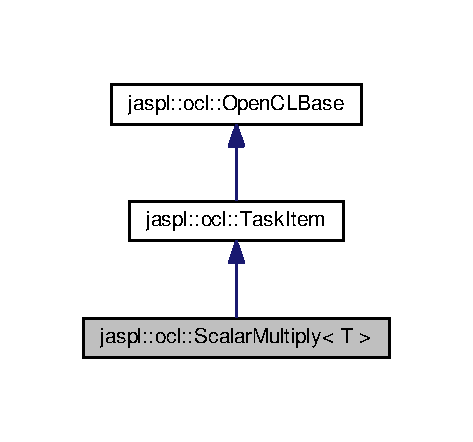
\includegraphics[width=227pt]{classjaspl_1_1ocl_1_1_scalar_multiply__inherit__graph}
\end{center}
\end{figure}


Collaboration diagram for jaspl\+:\+:ocl\+:\+:Scalar\+Multiply$<$ T $>$\+:\nopagebreak
\begin{figure}[H]
\begin{center}
\leavevmode
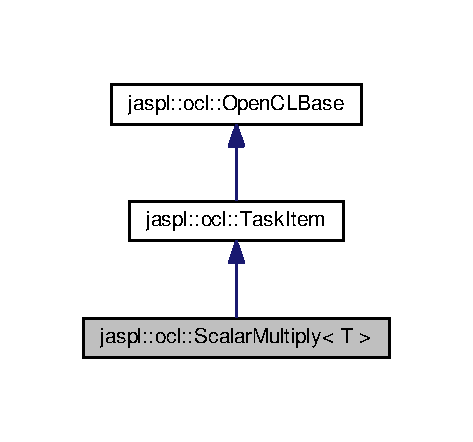
\includegraphics[width=227pt]{classjaspl_1_1ocl_1_1_scalar_multiply__coll__graph}
\end{center}
\end{figure}
\subsection*{Public Member Functions}
\begin{DoxyCompactItemize}
\item 
{\bfseries Scalar\+Multiply} (typename T\+::value\+\_\+type scalar\+\_\+value)\hypertarget{classjaspl_1_1ocl_1_1_scalar_multiply_a099a4868b984eea4d24c12c09933ee61}{}\label{classjaspl_1_1ocl_1_1_scalar_multiply_a099a4868b984eea4d24c12c09933ee61}

\end{DoxyCompactItemize}
\subsection*{Protected Member Functions}
\begin{DoxyCompactItemize}
\item 
void {\bfseries Trigger} ()\hypertarget{classjaspl_1_1ocl_1_1_scalar_multiply_a3797b44ad387b0bcd17413d11638d1c2}{}\label{classjaspl_1_1ocl_1_1_scalar_multiply_a3797b44ad387b0bcd17413d11638d1c2}

\item 
void {\bfseries Set\+Signal} (cl\+::\+Buffer \&signal\+\_\+buff, uint sig\+\_\+size)\hypertarget{classjaspl_1_1ocl_1_1_scalar_multiply_a21b27b0ec45a7327e6ddc25ea5f4d99a}{}\label{classjaspl_1_1ocl_1_1_scalar_multiply_a21b27b0ec45a7327e6ddc25ea5f4d99a}

\item 
cl\+::\+Buffer \& {\bfseries Processed\+Signal} ()\hypertarget{classjaspl_1_1ocl_1_1_scalar_multiply_acf198b3228d0b03e2c1ea12d67e387ff}{}\label{classjaspl_1_1ocl_1_1_scalar_multiply_acf198b3228d0b03e2c1ea12d67e387ff}

\item 
size\+\_\+t {\bfseries Processed\+Signal\+Bytes} ()\hypertarget{classjaspl_1_1ocl_1_1_scalar_multiply_a172e6495393f3d9b3618e471c103c95e}{}\label{classjaspl_1_1ocl_1_1_scalar_multiply_a172e6495393f3d9b3618e471c103c95e}

\item 
size\+\_\+t {\bfseries Processed\+Signal\+Size} ()\hypertarget{classjaspl_1_1ocl_1_1_scalar_multiply_ab76f39422e316fa67499cf07e8db7b4a}{}\label{classjaspl_1_1ocl_1_1_scalar_multiply_ab76f39422e316fa67499cf07e8db7b4a}

\item 
bool {\bfseries Needs\+To\+Reknew} ()\hypertarget{classjaspl_1_1ocl_1_1_scalar_multiply_a245ff6645743ee6e35d9977f68c3f70d}{}\label{classjaspl_1_1ocl_1_1_scalar_multiply_a245ff6645743ee6e35d9977f68c3f70d}

\end{DoxyCompactItemize}
\subsection*{Protected Attributes}
\begin{DoxyCompactItemize}
\item 
cl\+\_\+int {\bfseries err}\hypertarget{classjaspl_1_1ocl_1_1_scalar_multiply_a8e0f71ad2f0de06645b1f14e6ce9ec62}{}\label{classjaspl_1_1ocl_1_1_scalar_multiply_a8e0f71ad2f0de06645b1f14e6ce9ec62}

\end{DoxyCompactItemize}
\subsection*{Additional Inherited Members}


\subsection{Detailed Description}
\subsubsection*{template$<$class T$>$\\*
class jaspl\+::ocl\+::\+Scalar\+Multiply$<$ T $>$}



Definition at line 20 of file scalarmultiply.\+h.


\hypertarget{classjaspl_1_1ocl_1_1_task_item}{}\section{jaspl\+:\+:ocl\+:\+:Task\+Item Class Reference}
\label{classjaspl_1_1ocl_1_1_task_item}\index{jaspl\+::ocl\+::\+Task\+Item@{jaspl\+::ocl\+::\+Task\+Item}}


Inheritance diagram for jaspl\+:\+:ocl\+:\+:Task\+Item\+:\nopagebreak
\begin{figure}[H]
\begin{center}
\leavevmode
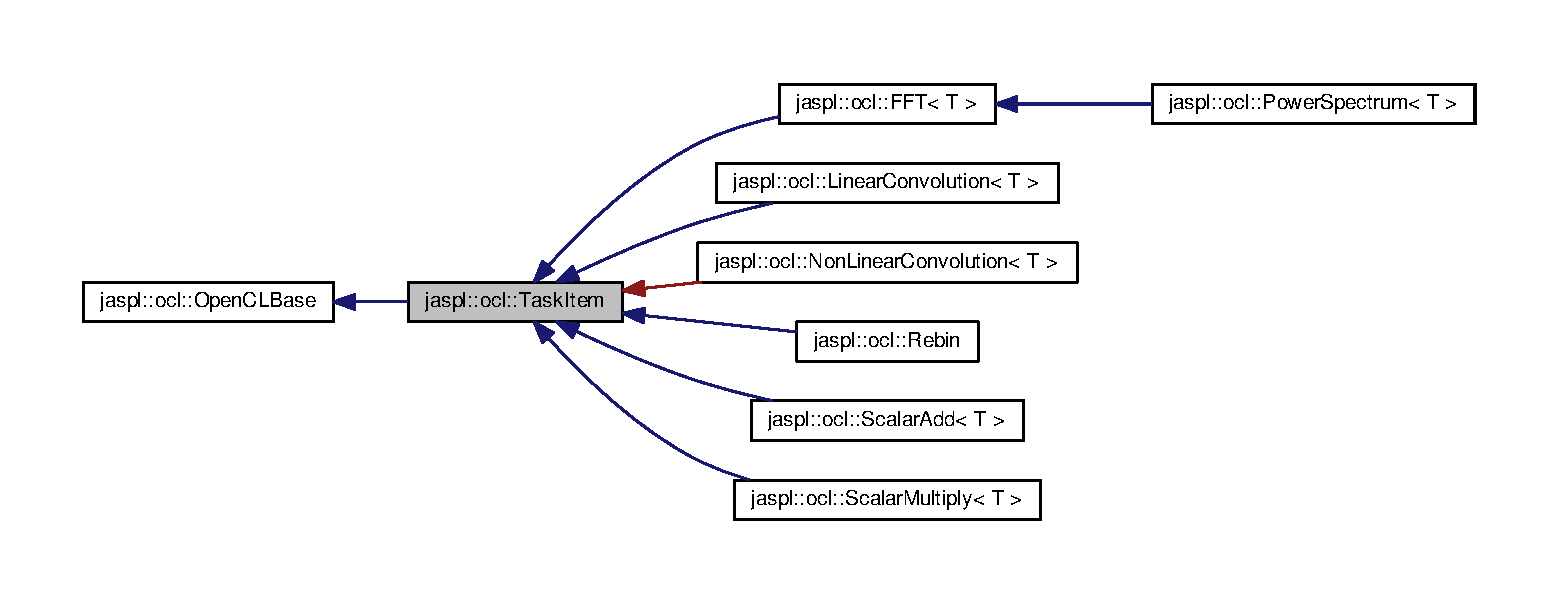
\includegraphics[width=350pt]{classjaspl_1_1ocl_1_1_task_item__inherit__graph}
\end{center}
\end{figure}


Collaboration diagram for jaspl\+:\+:ocl\+:\+:Task\+Item\+:\nopagebreak
\begin{figure}[H]
\begin{center}
\leavevmode
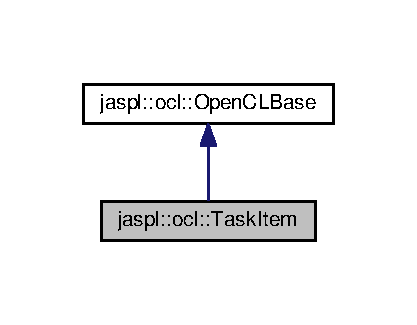
\includegraphics[width=200pt]{classjaspl_1_1ocl_1_1_task_item__coll__graph}
\end{center}
\end{figure}
\subsection*{Protected Member Functions}
\begin{DoxyCompactItemize}
\item 
{\footnotesize template$<$typename F $>$ }\\std\+::string {\bfseries Fake\+Kernel\+Templating} (std\+::string kernel\+\_\+source)\hypertarget{classjaspl_1_1ocl_1_1_task_item_aebceb791e8b1dbe70af39047d8fdae21}{}\label{classjaspl_1_1ocl_1_1_task_item_aebceb791e8b1dbe70af39047d8fdae21}

\item 
{\footnotesize template$<$typename F $>$ }\\void {\bfseries Load\+C\+L\+Kernel} (std\+::string kernel\+\_\+name)\hypertarget{classjaspl_1_1ocl_1_1_task_item_a800ffc9212ce8c25771e21b22ae867ce}{}\label{classjaspl_1_1ocl_1_1_task_item_a800ffc9212ce8c25771e21b22ae867ce}

\item 
virtual void {\bfseries Trigger} ()\hypertarget{classjaspl_1_1ocl_1_1_task_item_a186aa96ac98ce8bb8c63818e8b33e3fa}{}\label{classjaspl_1_1ocl_1_1_task_item_a186aa96ac98ce8bb8c63818e8b33e3fa}

\item 
virtual void {\bfseries Set\+Signal} (cl\+::\+Buffer \&signal\+\_\+buff, uint sig\+\_\+size)\hypertarget{classjaspl_1_1ocl_1_1_task_item_a906407a36a6dfb930b37eabaa612cea3}{}\label{classjaspl_1_1ocl_1_1_task_item_a906407a36a6dfb930b37eabaa612cea3}

\item 
virtual cl\+::\+Buffer \& {\bfseries Processed\+Signal} ()\hypertarget{classjaspl_1_1ocl_1_1_task_item_af607becf93865c5d3d8f3df6ef87f867}{}\label{classjaspl_1_1ocl_1_1_task_item_af607becf93865c5d3d8f3df6ef87f867}

\item 
virtual size\+\_\+t {\bfseries Processed\+Signal\+Bytes} ()\hypertarget{classjaspl_1_1ocl_1_1_task_item_ac82006308e53c6e42144d253bde9b535}{}\label{classjaspl_1_1ocl_1_1_task_item_ac82006308e53c6e42144d253bde9b535}

\item 
virtual size\+\_\+t {\bfseries Processed\+Signal\+Size} ()\hypertarget{classjaspl_1_1ocl_1_1_task_item_aface585662048bfa00cda3292e9d9273}{}\label{classjaspl_1_1ocl_1_1_task_item_aface585662048bfa00cda3292e9d9273}

\item 
virtual bool {\bfseries Needs\+To\+Reknew} ()\hypertarget{classjaspl_1_1ocl_1_1_task_item_a20e681f2c7b9930f99fc73ece96cb67c}{}\label{classjaspl_1_1ocl_1_1_task_item_a20e681f2c7b9930f99fc73ece96cb67c}

\item 
void {\bfseries Check\+Kernel\+Path} (std\+::string kernel\+\_\+source\+\_\+path)\hypertarget{classjaspl_1_1ocl_1_1_task_item_af048f07b953902e9ac048fb32dc86535}{}\label{classjaspl_1_1ocl_1_1_task_item_af048f07b953902e9ac048fb32dc86535}

\item 
std\+::string {\bfseries Get\+Open\+C\+L\+Source} (std\+::string kernel\+\_\+path)\hypertarget{classjaspl_1_1ocl_1_1_task_item_a015a0fc3c5fe671b6f9d529a77cb4132}{}\label{classjaspl_1_1ocl_1_1_task_item_a015a0fc3c5fe671b6f9d529a77cb4132}

\end{DoxyCompactItemize}
\subsection*{Protected Attributes}
\begin{DoxyCompactItemize}
\item 
std\+::string {\bfseries kernel\+\_\+path}\hypertarget{classjaspl_1_1ocl_1_1_task_item_aa08a1b3eaff97acd4083d81de0d78de9}{}\label{classjaspl_1_1ocl_1_1_task_item_aa08a1b3eaff97acd4083d81de0d78de9}

\item 
cl\+::\+Program\+::\+Sources {\bfseries sources}\hypertarget{classjaspl_1_1ocl_1_1_task_item_acf5a7b33791d535255f524dd7bdafa2d}{}\label{classjaspl_1_1ocl_1_1_task_item_acf5a7b33791d535255f524dd7bdafa2d}

\item 
std\+::string {\bfseries kernel\+\_\+source}\hypertarget{classjaspl_1_1ocl_1_1_task_item_a90439204dd331c6a4f488e3c6016ddfa}{}\label{classjaspl_1_1ocl_1_1_task_item_a90439204dd331c6a4f488e3c6016ddfa}

\item 
cl\+::\+Program {\bfseries program}\hypertarget{classjaspl_1_1ocl_1_1_task_item_afd9f6878a4a075d6fbc9cb2a74f3ac2e}{}\label{classjaspl_1_1ocl_1_1_task_item_afd9f6878a4a075d6fbc9cb2a74f3ac2e}

\item 
cl\+::\+Kernel {\bfseries kernel}\hypertarget{classjaspl_1_1ocl_1_1_task_item_ab628ae818420624811dee92ce68615fd}{}\label{classjaspl_1_1ocl_1_1_task_item_ab628ae818420624811dee92ce68615fd}

\item 
size\+\_\+t {\bfseries signal\+\_\+size}\hypertarget{classjaspl_1_1ocl_1_1_task_item_a8a21af3a15a0010ae139cc6b0555c380}{}\label{classjaspl_1_1ocl_1_1_task_item_a8a21af3a15a0010ae139cc6b0555c380}

\end{DoxyCompactItemize}
\subsection*{Friends}
\begin{DoxyCompactItemize}
\item 
class {\bfseries Task\+Queue\+Base}\hypertarget{classjaspl_1_1ocl_1_1_task_item_a7cef05d602ede8ae7e967835f6965bc7}{}\label{classjaspl_1_1ocl_1_1_task_item_a7cef05d602ede8ae7e967835f6965bc7}

\end{DoxyCompactItemize}
\subsection*{Additional Inherited Members}


\subsection{Detailed Description}


Definition at line 26 of file taskitem.\+h.


\hypertarget{classjaspl_1_1ocl_1_1_task_queue}{}\section{jaspl\+:\+:ocl\+:\+:Task\+Queue$<$ T $>$ Class Template Reference}
\label{classjaspl_1_1ocl_1_1_task_queue}\index{jaspl\+::ocl\+::\+Task\+Queue$<$ T $>$@{jaspl\+::ocl\+::\+Task\+Queue$<$ T $>$}}


Inheritance diagram for jaspl\+:\+:ocl\+:\+:Task\+Queue$<$ T $>$\+:\nopagebreak
\begin{figure}[H]
\begin{center}
\leavevmode
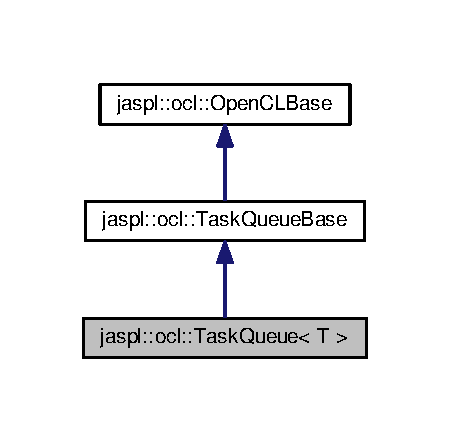
\includegraphics[width=216pt]{classjaspl_1_1ocl_1_1_task_queue__inherit__graph}
\end{center}
\end{figure}


Collaboration diagram for jaspl\+:\+:ocl\+:\+:Task\+Queue$<$ T $>$\+:\nopagebreak
\begin{figure}[H]
\begin{center}
\leavevmode
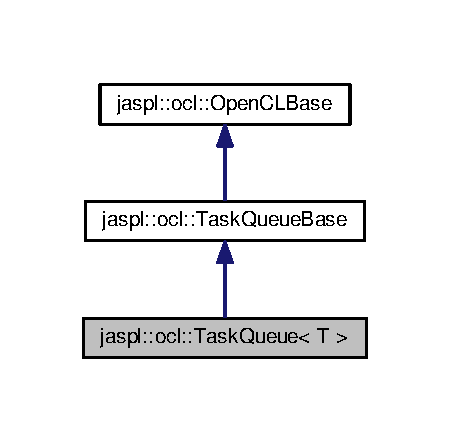
\includegraphics[width=216pt]{classjaspl_1_1ocl_1_1_task_queue__coll__graph}
\end{center}
\end{figure}
\subsection*{Public Member Functions}
\begin{DoxyCompactItemize}
\item 
{\bfseries Task\+Queue} (uint platform\+\_\+number, uint device\+\_\+number)\hypertarget{classjaspl_1_1ocl_1_1_task_queue_a622e6d731766740b8fde66c1e5dcc05d}{}\label{classjaspl_1_1ocl_1_1_task_queue_a622e6d731766740b8fde66c1e5dcc05d}

\item 
void {\bfseries Load} (T signal)\hypertarget{classjaspl_1_1ocl_1_1_task_queue_a66c6ece3e07f7eff2036bf0392606a59}{}\label{classjaspl_1_1ocl_1_1_task_queue_a66c6ece3e07f7eff2036bf0392606a59}

\item 
T {\bfseries Recall} ()\hypertarget{classjaspl_1_1ocl_1_1_task_queue_aada14bbe200a4e949cb647a20c46f22a}{}\label{classjaspl_1_1ocl_1_1_task_queue_aada14bbe200a4e949cb647a20c46f22a}

\end{DoxyCompactItemize}
\subsection*{Additional Inherited Members}


\subsection{Detailed Description}
\subsubsection*{template$<$typename T$>$\\*
class jaspl\+::ocl\+::\+Task\+Queue$<$ T $>$}



Definition at line 27 of file taskqueue.\+h.


\hypertarget{classjaspl_1_1ocl_1_1_task_queue_3_01_t_01_5_01_4}{}\section{jaspl\+:\+:ocl\+:\+:Task\+Queue$<$ T $\ast$ $>$ Class Template Reference}
\label{classjaspl_1_1ocl_1_1_task_queue_3_01_t_01_5_01_4}\index{jaspl\+::ocl\+::\+Task\+Queue$<$ T $\ast$ $>$@{jaspl\+::ocl\+::\+Task\+Queue$<$ T $\ast$ $>$}}


Inheritance diagram for jaspl\+:\+:ocl\+:\+:Task\+Queue$<$ T $\ast$ $>$\+:\nopagebreak
\begin{figure}[H]
\begin{center}
\leavevmode
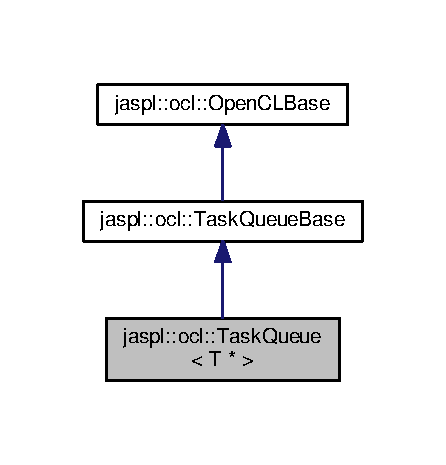
\includegraphics[width=214pt]{classjaspl_1_1ocl_1_1_task_queue_3_01_t_01_5_01_4__inherit__graph}
\end{center}
\end{figure}


Collaboration diagram for jaspl\+:\+:ocl\+:\+:Task\+Queue$<$ T $\ast$ $>$\+:\nopagebreak
\begin{figure}[H]
\begin{center}
\leavevmode
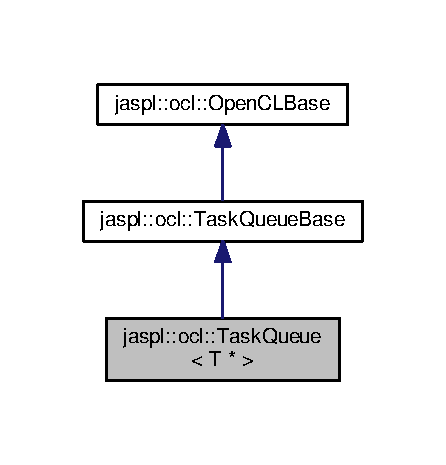
\includegraphics[width=214pt]{classjaspl_1_1ocl_1_1_task_queue_3_01_t_01_5_01_4__coll__graph}
\end{center}
\end{figure}
\subsection*{Public Member Functions}
\begin{DoxyCompactItemize}
\item 
{\bfseries Task\+Queue} (uint platform\+\_\+number, uint device\+\_\+number)\hypertarget{classjaspl_1_1ocl_1_1_task_queue_3_01_t_01_5_01_4_a79fad9fbd8502d2ad4fbc3bc72beb025}{}\label{classjaspl_1_1ocl_1_1_task_queue_3_01_t_01_5_01_4_a79fad9fbd8502d2ad4fbc3bc72beb025}

\item 
void {\bfseries Load} (T $\ast$signal\+\_\+ptr)\hypertarget{classjaspl_1_1ocl_1_1_task_queue_3_01_t_01_5_01_4_a551e195b02111e01482ef4a2783f5f1c}{}\label{classjaspl_1_1ocl_1_1_task_queue_3_01_t_01_5_01_4_a551e195b02111e01482ef4a2783f5f1c}

\item 
T $\ast$ {\bfseries Recall} ()\hypertarget{classjaspl_1_1ocl_1_1_task_queue_3_01_t_01_5_01_4_ab70f0e28df3b5b5217804a86d8f63994}{}\label{classjaspl_1_1ocl_1_1_task_queue_3_01_t_01_5_01_4_ab70f0e28df3b5b5217804a86d8f63994}

\end{DoxyCompactItemize}
\subsection*{Additional Inherited Members}


\subsection{Detailed Description}
\subsubsection*{template$<$class T$>$\\*
class jaspl\+::ocl\+::\+Task\+Queue$<$ T $\ast$ $>$}



Definition at line 39 of file taskqueue.\+h.


\hypertarget{classjaspl_1_1ocl_1_1_task_queue_base}{}\section{jaspl\+:\+:ocl\+:\+:Task\+Queue\+Base Class Reference}
\label{classjaspl_1_1ocl_1_1_task_queue_base}\index{jaspl\+::ocl\+::\+Task\+Queue\+Base@{jaspl\+::ocl\+::\+Task\+Queue\+Base}}


The fundamental structure underlying all Open\+CL Functions.  




{\ttfamily \#include $<$taskqueuebase.\+h$>$}



Inheritance diagram for jaspl\+:\+:ocl\+:\+:Task\+Queue\+Base\+:\nopagebreak
\begin{figure}[H]
\begin{center}
\leavevmode
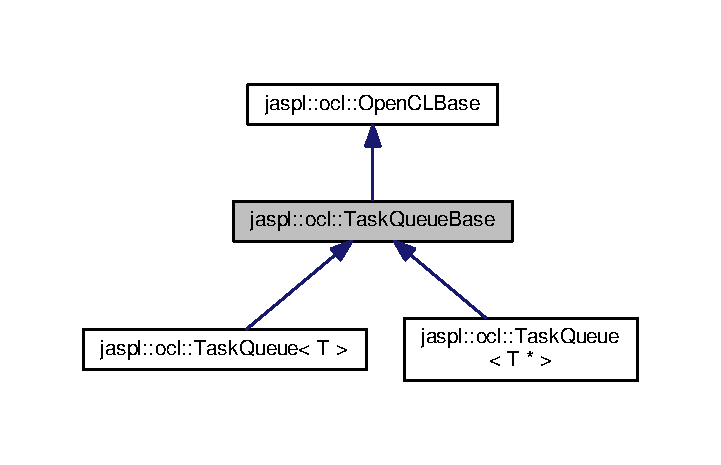
\includegraphics[width=346pt]{classjaspl_1_1ocl_1_1_task_queue_base__inherit__graph}
\end{center}
\end{figure}


Collaboration diagram for jaspl\+:\+:ocl\+:\+:Task\+Queue\+Base\+:\nopagebreak
\begin{figure}[H]
\begin{center}
\leavevmode
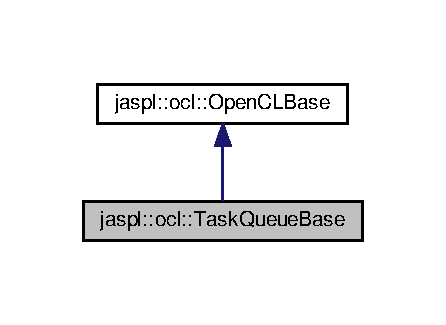
\includegraphics[width=214pt]{classjaspl_1_1ocl_1_1_task_queue_base__coll__graph}
\end{center}
\end{figure}
\subsection*{Public Member Functions}
\begin{DoxyCompactItemize}
\item 
\hyperlink{classjaspl_1_1ocl_1_1_task_queue_base_a6568c5c6bd8b3d2e2ad3c13eef6fb31b}{Task\+Queue\+Base} (uint platform\+\_\+number=0, uint device\+\_\+number=0)
\begin{DoxyCompactList}\small\item\em Build a new \hyperlink{classjaspl_1_1ocl_1_1_task_queue_base}{Task\+Queue\+Base} and implicitly initialize Open\+CL Context, Platform etc. \end{DoxyCompactList}\item 
void \hyperlink{classjaspl_1_1ocl_1_1_task_queue_base_af9671abc7d62d895bb6abdd9c68bb31c}{Execute} ()
\begin{DoxyCompactList}\small\item\em Run all Task\+Items that are currently loaded. \end{DoxyCompactList}\item 
void \hyperlink{classjaspl_1_1ocl_1_1_task_queue_base_aa71fb29536edbed03a771e40b81ea741}{Add\+Task\+Item} (\hyperlink{classjaspl_1_1ocl_1_1_task_item}{Task\+Item} \&item)
\begin{DoxyCompactList}\small\item\em Add a new \hyperlink{classjaspl_1_1ocl_1_1_task_item}{Task\+Item} into the \hyperlink{classjaspl_1_1ocl_1_1_task_queue}{Task\+Queue}. \end{DoxyCompactList}\item 
bool \hyperlink{classjaspl_1_1ocl_1_1_task_queue_base_a6415d52d4baca7807b251a6534f16b69}{Remove\+Task\+Item} (\hyperlink{classjaspl_1_1ocl_1_1_task_item}{Task\+Item} \&item)
\begin{DoxyCompactList}\small\item\em Remove a \hyperlink{classjaspl_1_1ocl_1_1_task_item}{Task\+Item} from the queue (if it exists) \end{DoxyCompactList}\item 
void \hyperlink{classjaspl_1_1ocl_1_1_task_queue_base_ac548bc47ba629093eb10c3566cb55d22}{Print\+Contents} ()\hypertarget{classjaspl_1_1ocl_1_1_task_queue_base_ac548bc47ba629093eb10c3566cb55d22}{}\label{classjaspl_1_1ocl_1_1_task_queue_base_ac548bc47ba629093eb10c3566cb55d22}

\begin{DoxyCompactList}\small\item\em Print all of the current elements in the queue in the order in which they will be executed. \end{DoxyCompactList}\item 
void {\bfseries Reknew\+Signal} (cl\+::\+Buffer \&processed\+\_\+buff, size\+\_\+t processed\+\_\+bytes, size\+\_\+t processed\+\_\+size)\hypertarget{classjaspl_1_1ocl_1_1_task_queue_base_a106853a7c3e48b1446013f6769e67a8a}{}\label{classjaspl_1_1ocl_1_1_task_queue_base_a106853a7c3e48b1446013f6769e67a8a}

\end{DoxyCompactItemize}
\subsection*{Protected Attributes}
\begin{DoxyCompactItemize}
\item 
std\+::list$<$ \hyperlink{classjaspl_1_1ocl_1_1_task_item}{Task\+Item} $\ast$ $>$ {\bfseries task\+\_\+queue}\hypertarget{classjaspl_1_1ocl_1_1_task_queue_base_a62a834cd1aa09f8387685a40bbe373c6}{}\label{classjaspl_1_1ocl_1_1_task_queue_base_a62a834cd1aa09f8387685a40bbe373c6}

\item 
cl\+::\+Buffer {\bfseries signal\+\_\+input}\hypertarget{classjaspl_1_1ocl_1_1_task_queue_base_ac9d244ae1978be6bb3fc806faf99f220}{}\label{classjaspl_1_1ocl_1_1_task_queue_base_ac9d244ae1978be6bb3fc806faf99f220}

\item 
cl\+::\+Buffer {\bfseries output}\hypertarget{classjaspl_1_1ocl_1_1_task_queue_base_aefa39df1b87a263a89b91ce5de343495}{}\label{classjaspl_1_1ocl_1_1_task_queue_base_aefa39df1b87a263a89b91ce5de343495}

\item 
size\+\_\+t {\bfseries signal\+\_\+size}\hypertarget{classjaspl_1_1ocl_1_1_task_queue_base_adbcead862a33ae1a246570a7e24cf786}{}\label{classjaspl_1_1ocl_1_1_task_queue_base_adbcead862a33ae1a246570a7e24cf786}

\item 
size\+\_\+t {\bfseries signal\+\_\+bytes}\hypertarget{classjaspl_1_1ocl_1_1_task_queue_base_a1e5ba37a36ce10e34822ddf5686d2971}{}\label{classjaspl_1_1ocl_1_1_task_queue_base_a1e5ba37a36ce10e34822ddf5686d2971}

\item 
bool {\bfseries on\+\_\+device} = false\hypertarget{classjaspl_1_1ocl_1_1_task_queue_base_a30d1e5405a0eb3732756a1bb6fd97c8d}{}\label{classjaspl_1_1ocl_1_1_task_queue_base_a30d1e5405a0eb3732756a1bb6fd97c8d}

\end{DoxyCompactItemize}
\subsection*{Friends}
\begin{DoxyCompactItemize}
\item 
class {\bfseries Task\+Item}\hypertarget{classjaspl_1_1ocl_1_1_task_queue_base_aec7aa930b50aea7c2192347a80371a14}{}\label{classjaspl_1_1ocl_1_1_task_queue_base_aec7aa930b50aea7c2192347a80371a14}

\end{DoxyCompactItemize}
\subsection*{Additional Inherited Members}


\subsection{Detailed Description}
The fundamental structure underlying all Open\+CL Functions. 

Definition at line 30 of file taskqueuebase.\+h.



\subsection{Constructor \& Destructor Documentation}
\index{jaspl\+::ocl\+::\+Task\+Queue\+Base@{jaspl\+::ocl\+::\+Task\+Queue\+Base}!Task\+Queue\+Base@{Task\+Queue\+Base}}
\index{Task\+Queue\+Base@{Task\+Queue\+Base}!jaspl\+::ocl\+::\+Task\+Queue\+Base@{jaspl\+::ocl\+::\+Task\+Queue\+Base}}
\subsubsection[{\texorpdfstring{Task\+Queue\+Base(uint platform\+\_\+number=0, uint device\+\_\+number=0)}{TaskQueueBase(uint platform_number=0, uint device_number=0)}}]{\setlength{\rightskip}{0pt plus 5cm}jaspl\+::ocl\+::\+Task\+Queue\+Base\+::\+Task\+Queue\+Base (
\begin{DoxyParamCaption}
\item[{uint}]{platform\+\_\+number = {\ttfamily 0}, }
\item[{uint}]{device\+\_\+number = {\ttfamily 0}}
\end{DoxyParamCaption}
)}\hypertarget{classjaspl_1_1ocl_1_1_task_queue_base_a6568c5c6bd8b3d2e2ad3c13eef6fb31b}{}\label{classjaspl_1_1ocl_1_1_task_queue_base_a6568c5c6bd8b3d2e2ad3c13eef6fb31b}


Build a new \hyperlink{classjaspl_1_1ocl_1_1_task_queue_base}{Task\+Queue\+Base} and implicitly initialize Open\+CL Context, Platform etc. 


\begin{DoxyParams}{Parameters}
{\em device\+\_\+number} & Number of the Open\+CL device to use as described by cl\+::\+Platform\+::get\+Devices(\+C\+L\+\_\+\+D\+E\+V\+I\+C\+E\+\_\+\+T\+Y\+P\+E\+\_\+\+A\+L\+L)\\
\hline
\end{DoxyParams}
Note that this will be the device that every \hyperlink{classjaspl_1_1ocl_1_1_task_item}{Task\+Item} will be executed on. 

Definition at line 18 of file taskqueuebase.\+cpp.



\subsection{Member Function Documentation}
\index{jaspl\+::ocl\+::\+Task\+Queue\+Base@{jaspl\+::ocl\+::\+Task\+Queue\+Base}!Add\+Task\+Item@{Add\+Task\+Item}}
\index{Add\+Task\+Item@{Add\+Task\+Item}!jaspl\+::ocl\+::\+Task\+Queue\+Base@{jaspl\+::ocl\+::\+Task\+Queue\+Base}}
\subsubsection[{\texorpdfstring{Add\+Task\+Item(\+Task\+Item \&item)}{AddTaskItem(TaskItem &item)}}]{\setlength{\rightskip}{0pt plus 5cm}void jaspl\+::ocl\+::\+Task\+Queue\+Base\+::\+Add\+Task\+Item (
\begin{DoxyParamCaption}
\item[{{\bf Task\+Item} \&}]{item}
\end{DoxyParamCaption}
)}\hypertarget{classjaspl_1_1ocl_1_1_task_queue_base_aa71fb29536edbed03a771e40b81ea741}{}\label{classjaspl_1_1ocl_1_1_task_queue_base_aa71fb29536edbed03a771e40b81ea741}


Add a new \hyperlink{classjaspl_1_1ocl_1_1_task_item}{Task\+Item} into the \hyperlink{classjaspl_1_1ocl_1_1_task_queue}{Task\+Queue}. 

Items added to the queue need not be unique, repeated Task\+Items are allowed.


\begin{DoxyParams}{Parameters}
{\em item} & The \hyperlink{classjaspl_1_1ocl_1_1_task_item}{Task\+Item} to be inserted into the queue. \\
\hline
\end{DoxyParams}


Definition at line 42 of file taskqueuebase.\+cpp.

\index{jaspl\+::ocl\+::\+Task\+Queue\+Base@{jaspl\+::ocl\+::\+Task\+Queue\+Base}!Execute@{Execute}}
\index{Execute@{Execute}!jaspl\+::ocl\+::\+Task\+Queue\+Base@{jaspl\+::ocl\+::\+Task\+Queue\+Base}}
\subsubsection[{\texorpdfstring{Execute()}{Execute()}}]{\setlength{\rightskip}{0pt plus 5cm}void jaspl\+::ocl\+::\+Task\+Queue\+Base\+::\+Execute (
\begin{DoxyParamCaption}
{}
\end{DoxyParamCaption}
)}\hypertarget{classjaspl_1_1ocl_1_1_task_queue_base_af9671abc7d62d895bb6abdd9c68bb31c}{}\label{classjaspl_1_1ocl_1_1_task_queue_base_af9671abc7d62d895bb6abdd9c68bb31c}


Run all Task\+Items that are currently loaded. 

Items are executed in the order in which they were added with \hyperlink{classjaspl_1_1ocl_1_1_task_queue_base_aa71fb29536edbed03a771e40b81ea741}{Add\+Task\+Item()}. 

Definition at line 22 of file taskqueuebase.\+cpp.

\index{jaspl\+::ocl\+::\+Task\+Queue\+Base@{jaspl\+::ocl\+::\+Task\+Queue\+Base}!Remove\+Task\+Item@{Remove\+Task\+Item}}
\index{Remove\+Task\+Item@{Remove\+Task\+Item}!jaspl\+::ocl\+::\+Task\+Queue\+Base@{jaspl\+::ocl\+::\+Task\+Queue\+Base}}
\subsubsection[{\texorpdfstring{Remove\+Task\+Item(\+Task\+Item \&item)}{RemoveTaskItem(TaskItem &item)}}]{\setlength{\rightskip}{0pt plus 5cm}bool jaspl\+::ocl\+::\+Task\+Queue\+Base\+::\+Remove\+Task\+Item (
\begin{DoxyParamCaption}
\item[{{\bf Task\+Item} \&}]{item}
\end{DoxyParamCaption}
)}\hypertarget{classjaspl_1_1ocl_1_1_task_queue_base_a6415d52d4baca7807b251a6534f16b69}{}\label{classjaspl_1_1ocl_1_1_task_queue_base_a6415d52d4baca7807b251a6534f16b69}


Remove a \hyperlink{classjaspl_1_1ocl_1_1_task_item}{Task\+Item} from the queue (if it exists) 


\begin{DoxyParams}{Parameters}
{\em item} & The \hyperlink{classjaspl_1_1ocl_1_1_task_item}{Task\+Item} to be removed.\\
\hline
\end{DoxyParams}
If item is not currently in the queue this function does nothing. \begin{DoxyReturn}{Returns}
true if item was removed, false otherwise. 
\end{DoxyReturn}


Definition at line 46 of file taskqueuebase.\+cpp.


%--- End generated contents ---

% Index
\backmatter
\newpage
\phantomsection
\clearemptydoublepage
\addcontentsline{toc}{chapter}{Index}
\printindex

\end{document}
